\chapter{Modelli lineari e K-nearest neighbors}\label{ch-05}

Dopo l'introduzione si passa ai primi modelli veri e propri, che
occupano due estremi opposti del panorama del ML. Da una parte i
\textbf{modelli lineari}: rigidi, con pochi parametri, fondati sulla
matematica classica ma già ricchi di concetti moderni (funzione di loss,
discesa del gradiente, regolarizzazione). Dall'altra il
\textbf{K-nearest neighbors}: estremamente flessibile, locale, senza un
vero modello da addestrare. Il confronto tra i due mostra concretamente
il compromesso tra flessibilità e controllo della complessità.

Con i modelli lineari si passa da uno spazio delle ipotesi discreto
(concept learning) a uno \textbf{continuo}, ancora ristretto ma
parametrizzato da numeri reali.

\section{Notazione sui dati}\label{notazione-sui-dati}

I dati sono organizzati in una matrice \(X\) di dimensione
\(l \times n\): \(l\) righe (i pattern, \(p = 1,\dots,l\)) e \(n\)
colonne (le feature, \(i = 1,\dots,n\)).

\begin{itemize}
\tightlist
\item
  \(\mathbf{x}\) (in grassetto) è un generico pattern, cioè una riga
  della tabella: esempio, istanza, campione, vettore di input;
\item
  \(x_i\) o \(x_j\) (scalare) è la componente \(i\) o \(j\) di un
  pattern \(\mathbf{x}\) (omettendo l'indice del pattern);
\item
  \(\mathbf{x}_p\) è il \(p\)-esimo pattern (riga);
\item
  \(x_{p,i}\), scritto anche \((\mathbf{x}_p)_i\), è la componente \(i\)
  del pattern \(p\);
\item
  per il target si usa \(y_p\) (o \(d_p\), \(t_p\)), con
  \(p = 1,\dots,l\).
\end{itemize}

Quando il contesto è chiaro alcuni indici vengono omessi.

\section{Modelli lineari}\label{modelli-lineari}

Il modello lineare è stato il pilastro della statistica. Come scrive
Hastie: \emph{``nonostante i grandi progressi delle moderne tecniche di
regressione non parametrica, i modelli lineari restano importanti, e
dobbiamo capirli bene''}. Si parte dalla forma più semplice, lineare
nelle variabili di input. Il modello lineare è anche una
\textbf{baseline} naturale: la prima domanda davanti a un problema è ``è
un problema lineare?''.

\subsection{Regressione lineare
univariata}\label{regressione-lineare-univariata}

Riprendiamo l'esercizio dell'introduzione: dati i punti \((1;\,2{,}1)\),
\((2;\,3{,}9)\), \((3;\,6{,}1)\), \((4;\,8{,}4)\), \((5;\,9{,}8)\)
avevamo ``indovinato'' \(h(x) = 2x\). Ora vogliamo trovare i parametri
in modo \textbf{sistematico}.

Nel caso univariato (una variabile di input \(x\), una di output \(y\))
si assume il modello \[
h_\mathbf{w}(x) = w_1 x + w_0,
\] dove \(w_0, w_1\) sono coefficienti reali detti \textbf{pesi}
(\emph{weights}) o parametri liberi. Si tratta di adattare ai dati una
retta. Lo spazio delle ipotesi è infinito (i \(\mathbf{w}\) sono
continui), ma la matematica classica fornisce una soluzione elegante che
risale a Gauss e Legendre (circa 1795). Sorprendentemente, con questo
strumento di base si può già ``apprendere'', e contiene molti concetti
rilevanti del ML moderno.

\subsubsection{Apprendimento tramite Least Mean
Squares}\label{apprendimento-tramite-least-mean-squares}

Addestrare significa trovare \(\mathbf{w}\) che \textbf{minimizza
l'errore empirico} sui dati di training: per ora ci concentriamo solo su
\(R_{emp}\) (il controllo della complessità verrà dopo). Dato un insieme
di \(l\) esempi \((x_p, y_p)\), cerchiamo
\(h_\mathbf{w}(x) = w_1 x + w_0\) che minimizza la \textbf{somma dei
quadrati dei residui}: \[
\text{Loss}(h_\mathbf{w}) = E(\mathbf{w}) = \sum_{p=1}^{l} \big(y_p - h_\mathbf{w}(x_p)\big)^2 = \sum_{p=1}^{l} \big(y_p - (w_1 x_p + w_0)\big)^2.
\] Per avere la media si divide per \(l\). È il metodo dei
\textbf{minimi quadrati} (\emph{Least (Mean) Squares}, LMS), cioè
\(\arg\min_\mathbf{w} E(\mathbf{w})\) in norma \(L^2\).

\begin{boxtip}{Perché i minimi quadrati?}

Ogni retta candidata produce dei \textbf{residui}, cioè le distanze
verticali tra i punti \((x_p, y_p)\) e la retta. Rette diverse hanno
residui diversi: minimizzare la somma dei loro quadrati è un modo
naturale di trovare la retta che meglio approssima i dati. In generale,
i minimi quadrati sono l'approccio standard per risolvere in modo
approssimato i \textbf{sistemi sovradeterminati}, cioè con più equazioni
(gli esempi) che incognite (i parametri).

\end{boxtip}

\subsubsection{Come si risolve}\label{come-si-risolve}

Un minimo locale è un \textbf{punto stazionario}, dove il gradiente è
nullo: \[
\frac{\partial E(\mathbf{w})}{\partial w_i} = 0, \qquad i = 1, \dots, n+1.
\] Nel caso semplice con due parametri si cercano \(w_0, w_1\) tali che
\(\frac{\partial E}{\partial w_0} = 0\) e
\(\frac{\partial E}{\partial w_1} = 0\). Poiché la loss è
\textbf{convessa} (una parabola in due dimensioni), non ci sono minimi
locali spuri e la soluzione esiste in forma chiusa: \[
w_1 = \frac{\sum_p x_p y_p - \frac{1}{l}\sum_p x_p \sum_p y_p}{\sum_p x_p^2 - \frac{1}{l}\left(\sum_p x_p\right)^2} = \frac{\operatorname{Cov}[x,y]}{\operatorname{Var}[x]}, \qquad w_0 = \bar{y} - w_1 \bar{x},
\] dove \(\bar{x} = \frac{1}{l}\sum_p x_p\) e
\(\bar{y} = \frac{1}{l}\sum_p y_p\) sono le medie.

\subsubsection{Calcolo del gradiente per un
pattern}\label{calcolo-del-gradiente-per-un-pattern}

Per un singolo pattern \((x, y)\), usando le regole di derivazione
(\(\frac{\partial k}{\partial w} = 0\),
\(\frac{\partial w}{\partial w} = 1\),
\(\frac{\partial f(w)^2}{\partial w} = 2 f(w) \frac{\partial f(w)}{\partial w}\),
e ``la derivata della somma è la somma delle derivate''): \[
\frac{\partial E(\mathbf{w})}{\partial w_i} = \frac{\partial (y - h_\mathbf{w}(x))^2}{\partial w_i} = 2\big(y - h_\mathbf{w}(x)\big) \frac{\partial \big(y - (w_1 x + w_0)\big)}{\partial w_i},
\] da cui \[
\frac{\partial E(\mathbf{w})}{\partial w_0} = -2\big(y - h_\mathbf{w}(x)\big), \qquad \frac{\partial E(\mathbf{w})}{\partial w_1} = -2\big(y - h_\mathbf{w}(x)\big)\, x.
\] La quantità \(\delta = y - h(x)\), l'errore sul pattern, verrà
chiamata \textbf{delta}. Per \(l\) pattern basta sommare; poi si estende
a input multidimensionali.

\begin{boxexample}{Esercizio svolto}

Con i dati \((1;2{,}1), (2;3{,}9), (3;6{,}1), (4;8{,}4), (5;9{,}8)\):
\(\bar x = 3\), \(\bar y = 6{,}06\);
\(\sum x_p y_p = 2{,}1 + 7{,}8 + 18{,}3 + 33{,}6 + 49 = 110{,}8\);
\(\sum x_p^2 = 55\). Quindi
\(w_1 = \frac{110{,}8 - 5 \cdot 3 \cdot 6{,}06}{55 - 45} = \frac{110{,}8 - 90{,}9}{10} = 1{,}99\)
e \(w_0 = 6{,}06 - 1{,}99 \cdot 3 = 0{,}09\). La retta trovata,
\(h(x) \approx 1{,}99x + 0{,}09\), conferma l'intuizione \(h(x) = 2x\).

\end{boxexample}

\subsection{Notazione per input
multidimensionali}\label{notazione-per-input-multidimensionali}

Con \(\mathbf{x}\) e \(\mathbf{w}\) vettori colonna, il modello lineare
è \[
\mathbf{w}^T\mathbf{x} + w_0 = w_0 + w_1 x_1 + w_2 x_2 + \dots + w_n x_n = w_0 + \sum_{i=1}^{n} w_i x_i.
\] \(w_0\) si chiama \textbf{intercetta}, soglia, \textbf{bias} o
offset. Conviene includere una componente costante \(x_0 = 1\)
nell'input, così che \[
\mathbf{x}^T = [1, x_1, \dots, x_n], \qquad \mathbf{w}^T = [w_0, w_1, \dots, w_n], \qquad h(\mathbf{x}_p) = \mathbf{x}_p^T\mathbf{w} = \sum_{i=0}^{n} x_{p,i} w_i.
\] Il modello lineare è quindi semplicemente un \textbf{prodotto
scalare} tra input e pesi. (Nelle reti neurali la trasposta viene spesso
omessa.)

\section{Classificazione con modelli
lineari}\label{classificazione-con-modelli-lineari}

\subsection{Il problema}\label{il-problema}

Consideriamo 200 punti in \(\mathbb{R}^2\), generati da una
distribuzione sconosciuta, 100 per ciascuna di due classi. Possiamo
costruire una regola che predica il colore di punti futuri? I dati
potrebbero essere generati da una gaussiana per classe (con medie
diverse), oppure da una miscela di tante gaussiane a bassa varianza.

\begin{figure}[htbp]
\centering
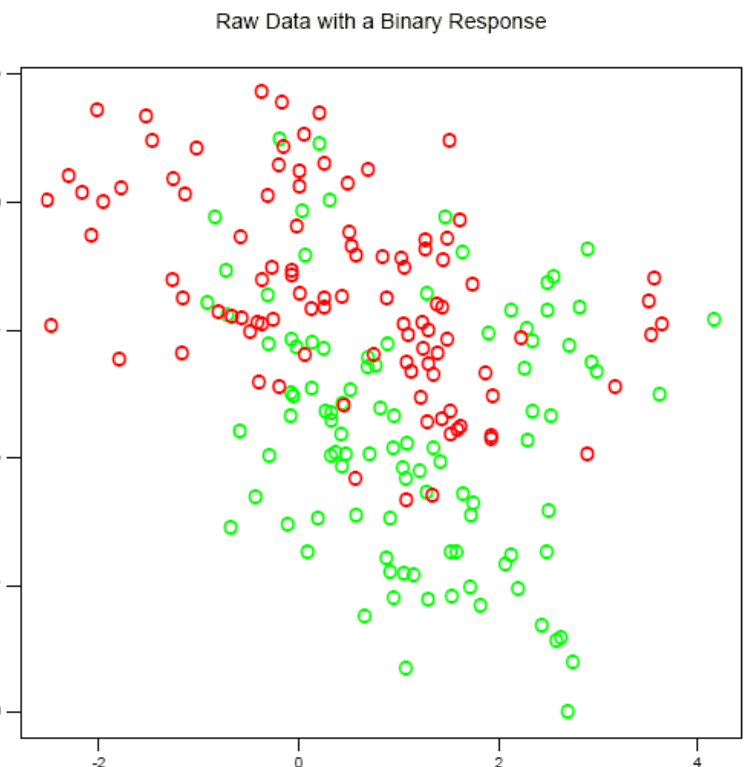
\includegraphics[width=0.43\linewidth,height=0.42\textheight,keepaspectratio]{images/05-lin_dataset.png}
\caption{Il problema di esempio (Hastie-Tibshirani-Friedman): 200 punti di due
classi.}
\end{figure}

\subsection{Iperpiani e regioni di
decisione}\label{iperpiani-e-regioni-di-decisione}

Gli stessi modelli usati per la regressione possono essere usati per la
\textbf{classificazione}, con target categorici (\(0/1\) o \(-1/+1\)).
L'espressione \(\mathbf{w}^T\mathbf{x}\) definisce un
\textbf{iperpiano}; si sfrutta il fatto che \(\mathbf{w}^T\mathbf{x}\)
assume valori positivi da un lato e negativi dall'altro per decidere a
quale classe appartiene un punto. L'obiettivo è trovare, tramite
l'apprendimento, un \(\mathbf{w}\) che dia una buona accuratezza.

In due dimensioni,
\(\mathbf{w}^T\mathbf{x} = w_0 + w_1 x_1 + w_2 x_2 = 0\) è una retta: il
\textbf{confine di decisione} (\emph{decision boundary}).

\begin{figure}[htbp]
\centering
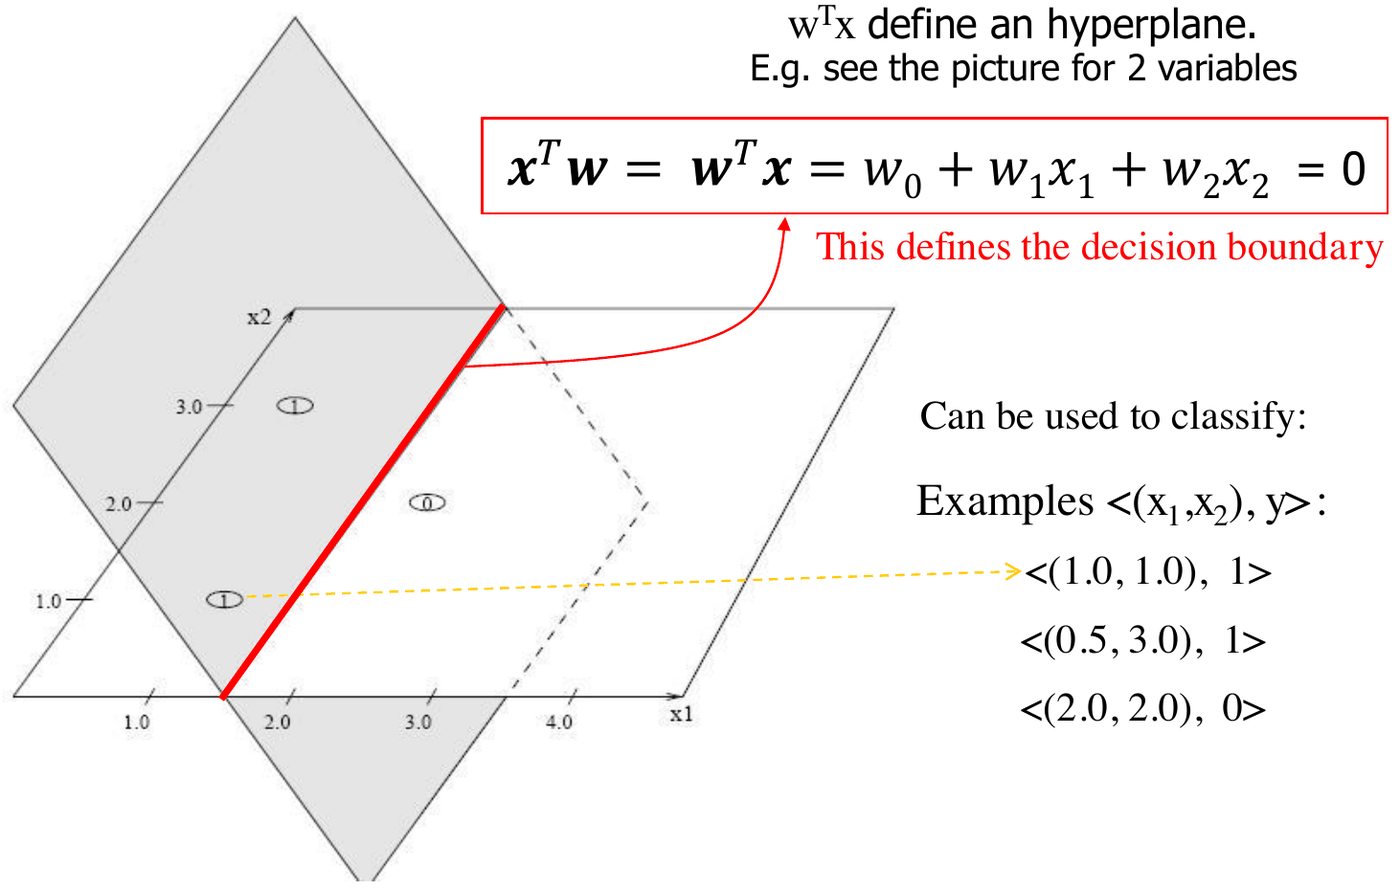
\includegraphics[width=0.71\linewidth,height=0.42\textheight,keepaspectratio]{images/05-lin_iperpiano.png}
\caption{L'iperpiano \(\mathbf{w}^T\mathbf{x}\) e la sua intersezione con il
piano degli input: il confine di decisione.}
\end{figure}

Per ottenere un classificatore si applica una \textbf{funzione soglia}:
\[
h(\mathbf{x}) = \begin{cases} 1 & \text{se } \mathbf{w}^T\mathbf{x} + w_0 \ge 0 \\ 0 & \text{altrimenti} \end{cases} \quad \text{(output in } [0,1]\text{)}, \qquad h(\mathbf{x}) = \operatorname{sign}(\mathbf{w}^T\mathbf{x} + w_0) \quad \text{(output in } [-1,+1]\text{)}.
\] Includendo \(w_0\) in \(\mathbf{w}\):
\(h(\mathbf{x}_p) = \operatorname{sign}(\mathbf{x}_p^T\mathbf{w}) = \operatorname{sign}\left(\sum_{i=0}^{n} x_{p,i} w_i\right)\).
È la \textbf{Linear Threshold Unit} (LTU).

\begin{boxnote}{Il bias come soglia}

Dire \(\mathbf{w}^T\mathbf{x} + w_0 \ge 0\) equivale a dire
\(\mathbf{w}^T\mathbf{x} \ge -w_0\). Le due forme individuano la stessa
regione positiva, ma la seconda mette in evidenza il ruolo del bias:
\(-w_0\) è il \textbf{valore di soglia} che la combinazione pesata degli
input deve superare per ``attivare'' l'uscita \(+1\).

\end{boxnote}

\subsection{Usare il modello: due
esempi}\label{usare-il-modello-due-esempi}

\begin{boxexample}{Terremoti o esplosioni nucleari? (AIMA)}

Dati sismici (1982--1990, Asia): \(x_1\) è la magnitudo delle onde di
volume, \(x_2\) quella delle onde di superficie. Un algoritmo di
apprendimento trova il confine \(-4{,}9 + 1{,}7x_1 - x_2 = 0\). Per
classificare un nuovo evento \((6, 3)\): \[
h(6,3) = \operatorname{sign}(-4{,}9 + 1{,}7 \cdot 6 - 1 \cdot 3) = \operatorname{sign}(2{,}3) = +1 \;\Rightarrow\; \text{esplosione nucleare.}
\] (Ottenere nuovi esempi di training, in questo caso, è decisamente
costoso.)

\end{boxexample}

\begin{figure}[htbp]
\centering
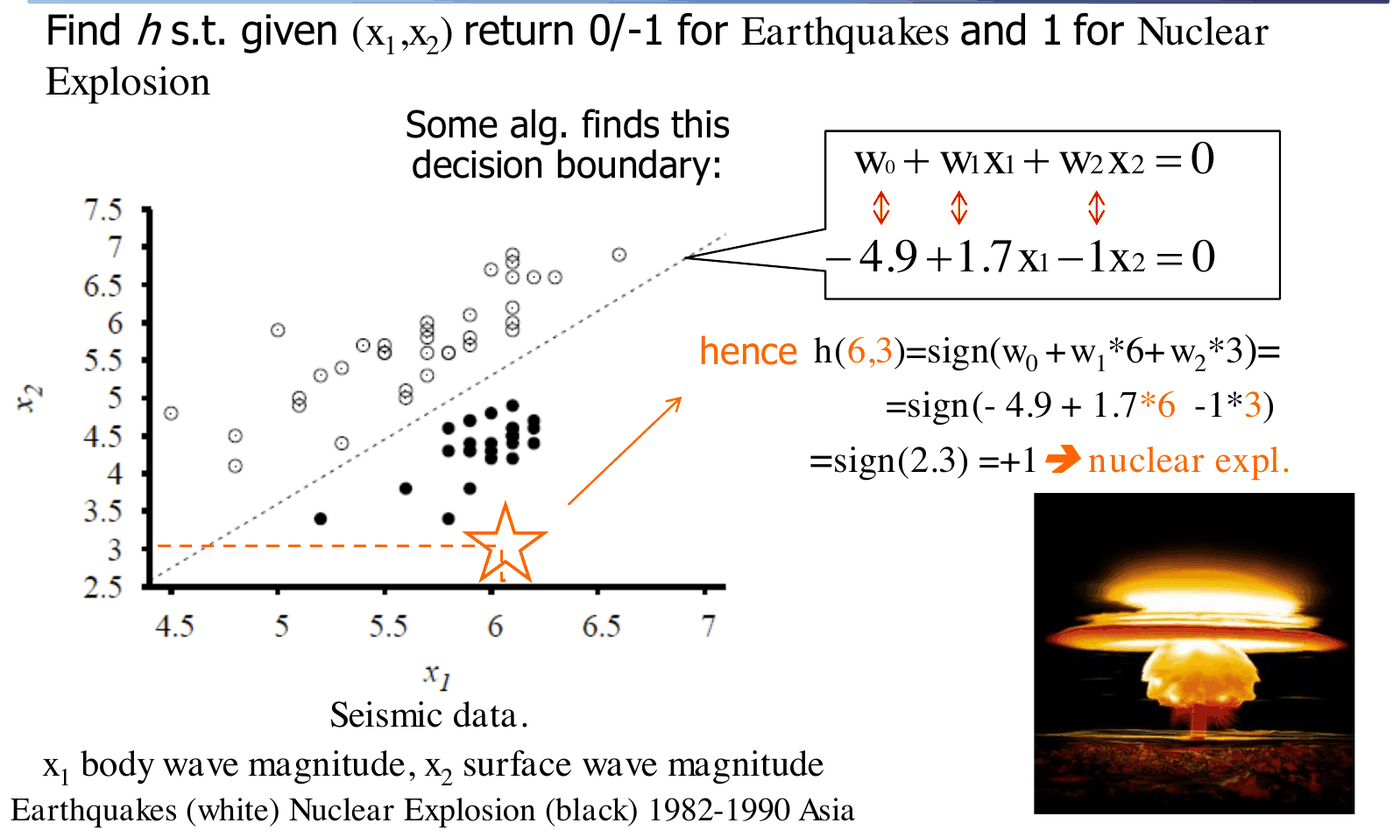
\includegraphics[width=0.80\linewidth,height=0.42\textheight,keepaspectratio]{images/05-lin_aima-sismi.png}
\caption{Classificazione di dati sismici con un confine di decisione lineare.}
\end{figure}

\begin{boxexample}{Filtro antispam}

Si vuole \(h(\text{mail}) = +1\) per lo spam e \(-1\) altrimenti. Le
feature \(\phi_k(\text{mail})\) sono ad esempio la presenza (\(0/1\)) di
parole o frasi (``free money'') o la lunghezza (intero): è la
rappresentazione \emph{bag of words}. Ogni peso \(w_k\) esprime il
contributo della feature alla predizione: positivo per ``free money'',
negativo per ``.edu'' o ``unipi''. La classificazione è
\(h_\mathbf{w}(\mathbf{x}) = \operatorname{sign}\left(\sum_k w_k \phi_k(\mathbf{x})\right)\):
se la combinazione pesata è positiva, è spam.

\end{boxexample}

\subsection{Proprietà utili
dell'iperpiano}\label{proprietuxe0-utili-delliperpiano}

\begin{figure}[htbp]
\centering
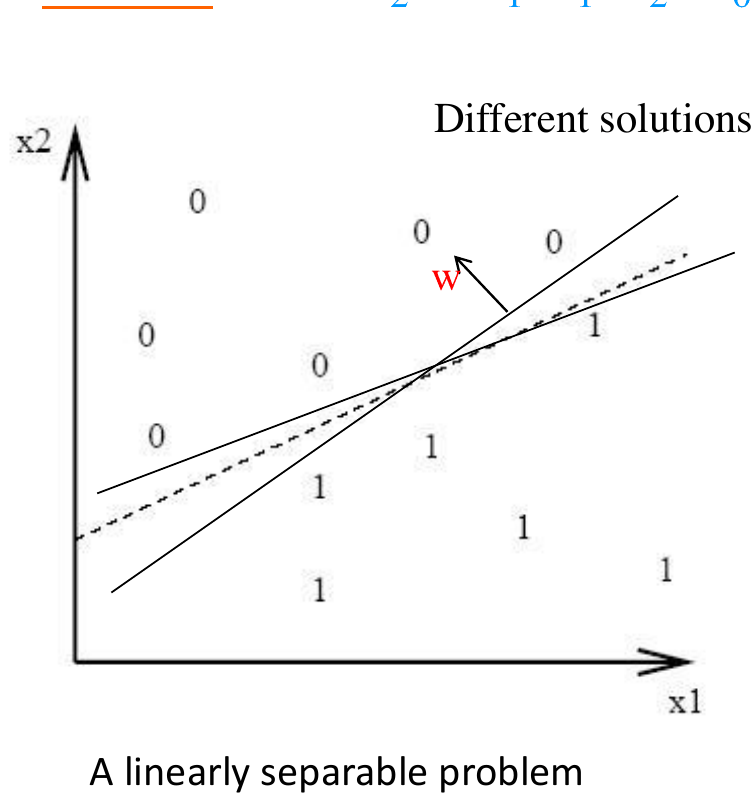
\includegraphics[width=0.43\linewidth,height=0.42\textheight,keepaspectratio]{images/05-lin_proprieta.png}
\caption{Un problema linearmente separabile ammette molti iperpiani separatori;
\(\mathbf{w}\) è ortogonale all'iperpiano.}
\end{figure}

\begin{itemize}
\tightlist
\item
  Se \(w_0 = 0\) la retta passa per l'\textbf{origine}.
\item
  Se \(n > 2\) il confine è un \textbf{iperpiano}.
\item
  \textbf{Libertà di scala}: moltiplicando \(\mathbf{w}\) per una
  costante \(K\) il confine non cambia.
\item
  \textbf{\(\mathbf{w}\) è ortogonale all'iperpiano}: presi due punti
  \(\mathbf{x}_a, \mathbf{x}_b\) sull'iperpiano,
  \(\mathbf{w}^T\mathbf{x}_a + w_0 = 0\) e
  \(\mathbf{w}^T\mathbf{x}_b + w_0 = 0\); sottraendo si ha
  \(\mathbf{w}^T(\mathbf{x}_a - \mathbf{x}_b) = 0\), cioè \(\mathbf{w}\)
  è ortogonale a ogni vettore che giace sull'iperpiano.
\item
  Se esiste un iperpiano separatore, \textbf{ne esistono molti}, e
  quindi anche molti algoritmi per trovarli.
\end{itemize}

L'equazione della retta si può riscrivere come
\(x_2 = -x_1 \frac{w_1}{w_2} - \frac{w_0}{w_2}\): provare a disegnarla
con valori diversi di \(\mathbf{w}\) è un buon esercizio.

\section{Il problema di
apprendimento}\label{il-problema-di-apprendimento}

\subsection{Formulazione}\label{formulazione}

Dati \(l\) esempi \((\mathbf{x}_p, y_p)\) con \(y_p \in \{0,1\}\) o
\(\{-1,+1\}\) e una loss \(L\), si cerca \(\mathbf{w}\) che minimizzi il
rischio empirico \[
R_{emp} = \frac{1}{l}\sum_{p=1}^{l} L\big(h(\mathbf{x}_p), y_p\big).
\] Per la classificazione, usare direttamente la loss 0/1 su
\(\operatorname{sign}(\mathbf{w}^T\mathbf{x})\) rende il problema
difficile: la funzione è \textbf{costante a tratti}, quindi il gradiente
è zero quasi ovunque e non dà indicazioni su come muoversi, e si finisce
in problemi combinatori.

\subsection{Sostituire la loss con una funzione
liscia}\label{sostituire-la-loss-con-una-funzione-liscia}

L'idea è sostituire la loss 0/1 con una funzione \textbf{liscia e
differenziabile}, come l'errore quadratico, applicata direttamente
all'uscita lineare \(\mathbf{w}^T\mathbf{x}\) (non a \(h(\mathbf{x})\),
che contiene il segno): \[
E(\mathbf{w}) = \sum_{p=1}^{l}(y_p - \mathbf{x}_p^T\mathbf{w})^2 = \|\mathbf{y} - X\mathbf{w}\|^2.
\]

\begin{figure}[htbp]
\centering
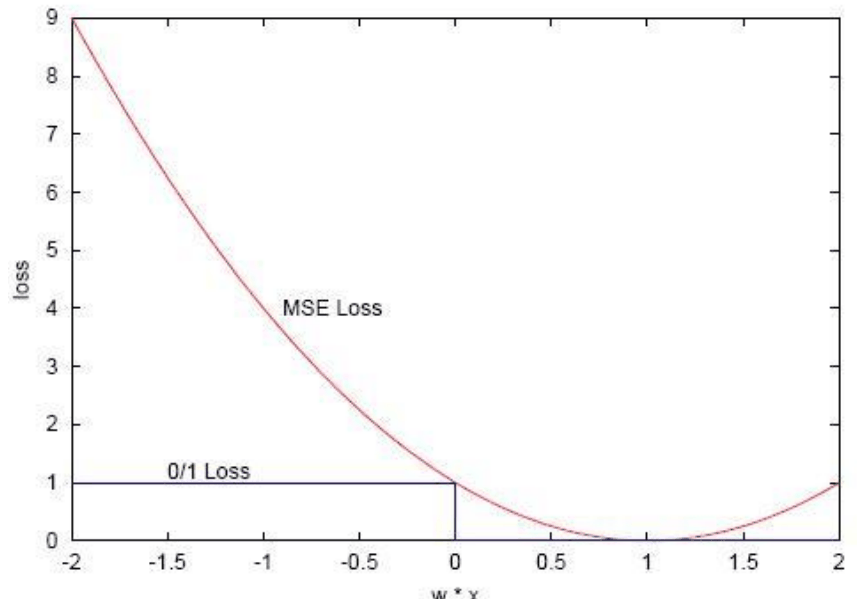
\includegraphics[width=0.54\linewidth,height=0.42\textheight,keepaspectratio]{images/05-lin_loss-smooth.png}
\caption{Loss 0/1 e loss quadratica per un pattern con target \(y = 1\): entrambe
sono minimizzate nella zona \(\mathbf{w}^T\mathbf{x} > 0\).}
\end{figure}

Perché funziona? Con target \(y_p = 1\), minimizzare
\((1 - \mathbf{x}_p^T\mathbf{w})^2\) spinge \(\mathbf{x}_p^T\mathbf{w}\)
verso \(1\), quindi positivo: niente errore di classificazione. Con
\(y_p = -1\) lo spinge verso \(-1\). Entrambe le loss sono minimizzate
nella stessa zona (a destra nel grafico). La funzione è
\textbf{quadratica}, quindi un minimo esiste sempre (ma non è
necessariamente unico). Lo stesso approccio vale identico per la
regressione.

Si vedono ora due algoritmi di apprendimento, entrambi basati su LMS e
validi sia per regressione sia per classificazione:

\begin{enumerate}
\def\labelenumi{\arabic{enumi}.}
\tightlist
\item
  un \textbf{approccio diretto} basato sulle \textbf{equazioni normali};
\item
  un \textbf{approccio iterativo} basato sulla \textbf{discesa del
  gradiente}.
\end{enumerate}

\subsection{Approccio diretto: le equazioni
normali}\label{approccio-diretto-le-equazioni-normali}

Derivando \(E(\mathbf{w})\) rispetto alla componente \(w_j\): \[
\frac{\partial E(\mathbf{w})}{\partial w_j} = \sum_{p=1}^{l} 2(y_p - \mathbf{x}_p^T\mathbf{w}) \frac{\partial (y_p - \mathbf{x}_p^T\mathbf{w})}{\partial w_j}.
\] Nel prodotto scalare
\(\mathbf{x}_p^T\mathbf{w} = x_{p,1}w_1 + x_{p,2}w_2 + \dots\) l'unico
termine che dipende da \(w_j\) è \(x_{p,j}w_j\), la cui derivata è
\(x_{p,j}\). Quindi: \[
\frac{\partial E(\mathbf{w})}{\partial w_j} = -2\sum_{p=1}^{l} (y_p - \mathbf{x}_p^T\mathbf{w})\, x_{p,j} = -2\sum_{p=1}^{l} \delta_p\, x_{p,j},
\] dove \(\delta_p = y_p - \mathbf{x}_p^T\mathbf{w}\) è l'errore sul
pattern \(p\). Questa forma tornerà nelle reti neurali.

Imponendo il gradiente nullo e passando in notazione matriciale si
ottengono le \textbf{equazioni normali}: \[
(X^T X)\,\mathbf{w} = X^T \mathbf{y}.
\]

\begin{boxtheorem}{Soluzione ai minimi quadrati}

Se \(X^TX\) è non singolare, la soluzione è unica: \[
\mathbf{w} = (X^TX)^{-1}X^T\mathbf{y} = X^+\mathbf{y},
\] dove \(X^+\) è la \textbf{pseudoinversa di Moore-Penrose} (definita
anche se \(X\) non è invertibile). Altrimenti le soluzioni sono
infinite, e si può scegliere quella a \textbf{norma minima} di
\(\mathbf{w}\).

\end{boxtheorem}

In pratica si usa la \textbf{decomposizione ai valori singolari} (SVD):
\(X = U\Sigma V^T\) implica \(X^+ = V\Sigma^+U^T\), dove \(\Sigma^+\) si
ottiene sostituendo ogni elemento diagonale non nullo con il suo
reciproco. Applicando la SVD si calcola direttamente
\(\mathbf{w} = X^+\mathbf{y}\), ottenendo la soluzione a norma minima.
\textbf{Questo è l'algoritmo di apprendimento} dell'approccio diretto; è
implementato in tutte le librerie numeriche (Numerical Recipes,
Armadillo, NumPy, R, Matlab\ldots), con molte varianti per efficienza e
stabilità.

\subsection{Approccio iterativo: la discesa del
gradiente}\label{approccio-iterativo-la-discesa-del-gradiente}

Perché cercare altri approcci se esiste la soluzione diretta? Un
approccio iterativo permette di ottenere:

\begin{itemize}
\tightlist
\item
  soluzioni \textbf{più efficienti} (quella diretta è cubica nella
  dimensione della matrice);
\item
  \textbf{regolarizzazione} (per ridurre la complessità del modello);
\item
  migliore approssimazione con dati rumorosi, fermando la ricerca
  \textbf{prima del minimo};
\item
  soprattutto, un metodo applicabile anche a \textbf{modelli non
  lineari}. È la base degli approcci fondamentali che vedremo (reti
  neurali).
\end{itemize}

\subsubsection{L'idea}\label{lidea}

Il gradiente
\(\frac{\partial E}{\partial w_j} = -2\sum_p (y_p - \mathbf{x}_p^T\mathbf{w})\, x_{p,j}\)
indica la direzione di \textbf{salita} dell'errore. Muovendosi nel verso
opposto (\(\Delta\mathbf{w} = -\nabla E(\mathbf{w})\)) si scende verso
il minimo. È una \textbf{ricerca locale}: si parte da un vettore di pesi
iniziale e lo si modifica iterativamente per diminuire l'errore
(\emph{steepest descent}).

\begin{figure}[htbp]
\centering
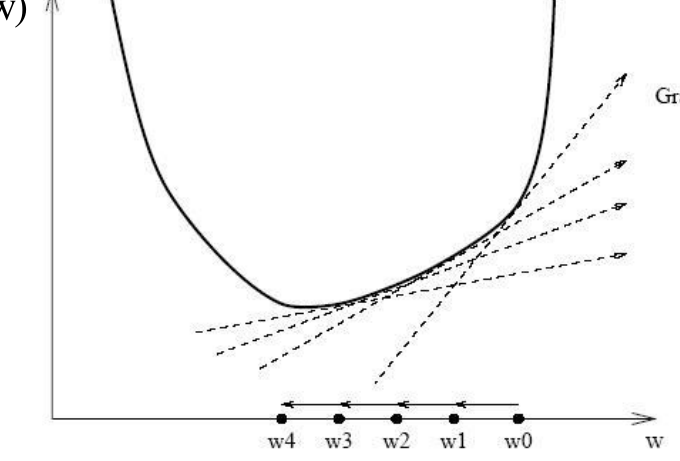
\includegraphics[width=0.46\linewidth,height=0.42\textheight,keepaspectratio]{images/05-lin_discesa-1d.png}
\caption{Discesa del gradiente in una dimensione: a ogni passo il peso si sposta
nel verso opposto alla pendenza.}
\end{figure}

Con due pesi, la superficie d'errore \(E([w_0, w_1]^T)\) è un
\textbf{paraboloide} (funzione quadratica convessa), e il gradiente
negativo è la nostra ``bussola'' per trovare il minimo.

\begin{figure}[htbp]
\centering
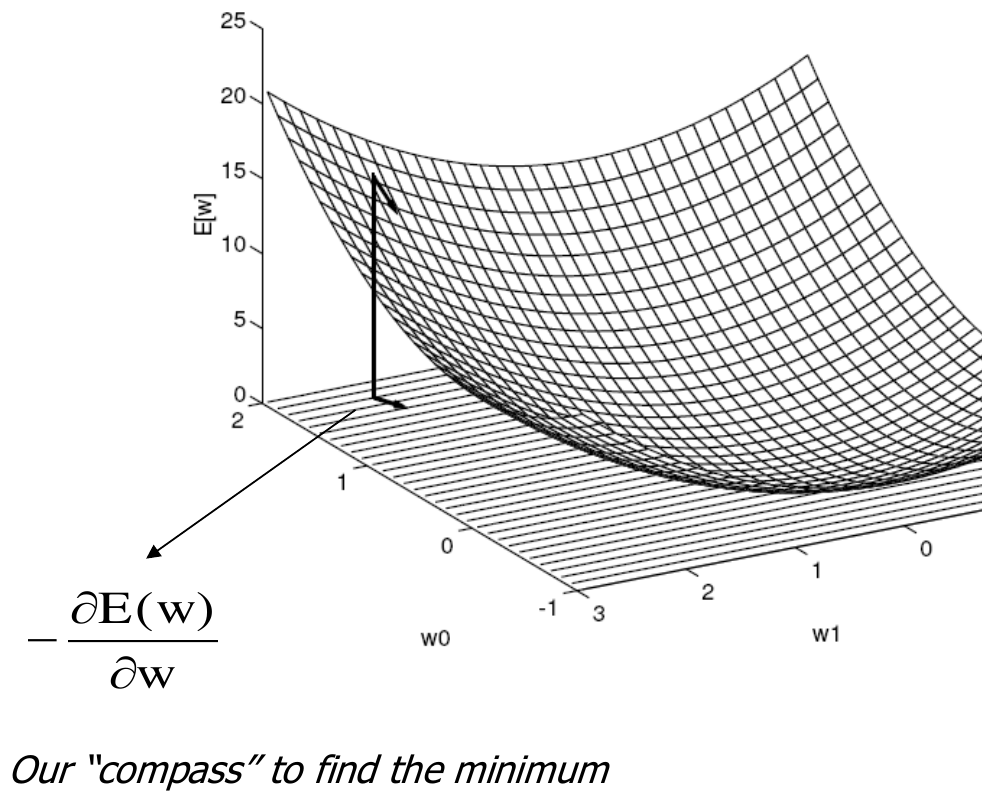
\includegraphics[width=0.54\linewidth,height=0.42\textheight,keepaspectratio]{images/05-lin_superficie-errore.png}
\caption{La superficie d'errore di un modello lineare con due pesi: ogni punto
del piano \((w_0, w_1)\) è un'ipotesi.}
\end{figure}

In generale il vettore \(\Delta\mathbf{w}\) ha una componente per ogni
peso: \[
\Delta\mathbf{w} = -\frac{\partial E(\mathbf{w})}{\partial \mathbf{w}} = \left( -\frac{\partial E}{\partial w_0}, -\frac{\partial E}{\partial w_1}, \dots, -\frac{\partial E}{\partial w_n} \right)^T,
\] e si può lavorare in spazi multidimensionali senza bisogno di
visualizzarli.

\subsubsection{La regola di apprendimento (delta
rule)}\label{la-regola-di-apprendimento-delta-rule}

Ci si muove iterativamente con una \textbf{regola di apprendimento}: \[
\mathbf{w}_{new} = \mathbf{w} + \eta\, \Delta\mathbf{w},
\] dove \(\eta\) (eta) è il \textbf{learning rate} (\emph{step size}),
che regola la velocità della discesa.

\begin{boxabstract}{Algoritmo di discesa del gradiente}

\begin{enumerate}
\def\labelenumi{\arabic{enumi}.}
\tightlist
\item
  Inizializzare \(\mathbf{w}\) con valori piccoli; fissare
  \(0 < \eta < 1\).
\item
  Calcolare
  \(\Delta\mathbf{w} = -\frac{\partial E(\mathbf{w})}{\partial \mathbf{w}}\).
\item
  Aggiornare \(\mathbf{w}_{new} = \mathbf{w} + \eta\,\Delta\mathbf{w}\).
\item
  Ripetere dal passo 2 fino a convergenza o finché \(E(\mathbf{w})\) è
  ``abbastanza piccolo''.
\end{enumerate}

\end{boxabstract}

Note:

\begin{itemize}
\tightlist
\item
  usare \(\Delta\mathbf{w}/l\) corrisponde al \emph{least mean squares}
  (dividere per \(l\) sarà il caso standard);
\item
  \(\eta\) regola un compromesso \textbf{velocità/stabilità}; può essere
  ridotto gradualmente verso zero per garantire la convergenza evitando
  oscillazioni attorno al minimo (molte varianti verranno viste più
  avanti).
\end{itemize}

\subsubsection{Batch e on-line}\label{batch-e-on-line}

\begin{itemize}
\tightlist
\item
  \textbf{Versione batch}: il gradiente è la somma su \textbf{tutti} gli
  \(l\) pattern, e i pesi si aggiornano dopo aver visto tutto il
  training set (un'\textbf{epoca}). La stima del gradiente è più
  ``precisa''.
\item
  \textbf{Versione on-line} (o \textbf{stocastica}, SGD): i pesi si
  aggiornano dopo \textbf{ogni} pattern, con il gradiente del singolo
  pattern: \[
  \frac{\partial E_p(\mathbf{w})}{\partial w_j} = -2(y_p - \mathbf{x}_p^T\mathbf{w})\, x_{p,j} = -\Delta_p w_j.
  \] L'output del secondo pattern è quindi calcolato con pesi già
  aggiornati dal primo, e così via. Fa progressi a ogni esempio, può
  essere più veloce, ma richiede un \(\eta\) più piccolo.
\end{itemize}

Esistono casi intermedi (\textbf{mini-batch}), che vedremo più avanti.

\begin{figure}[htbp]
\centering
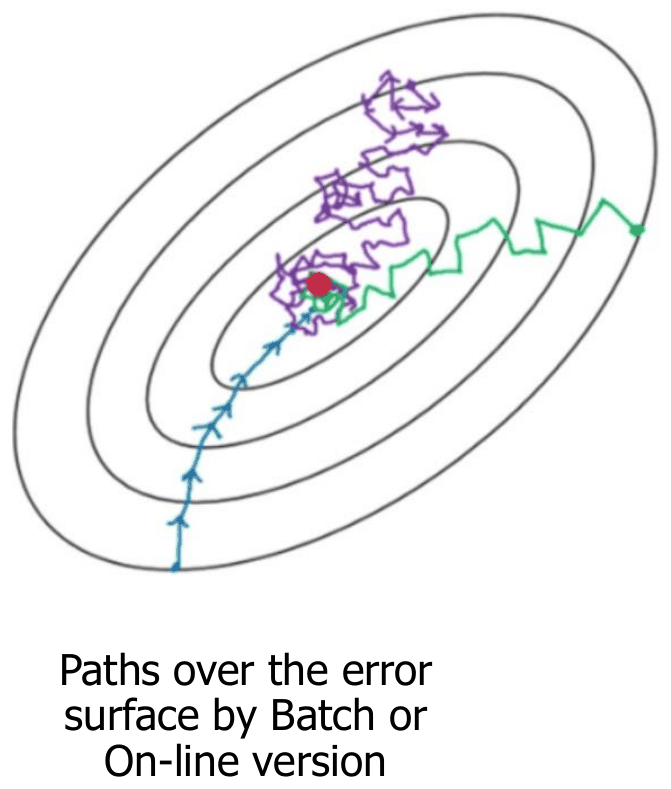
\includegraphics[width=0.40\linewidth,height=0.42\textheight,keepaspectratio]{images/05-lin_batch-online.png}
\caption{Percorsi sulla superficie d'errore: batch (blu, regolare) e on-line
(viola e verde, più irregolari).}
\end{figure}

\begin{figure}[htbp]
\centering
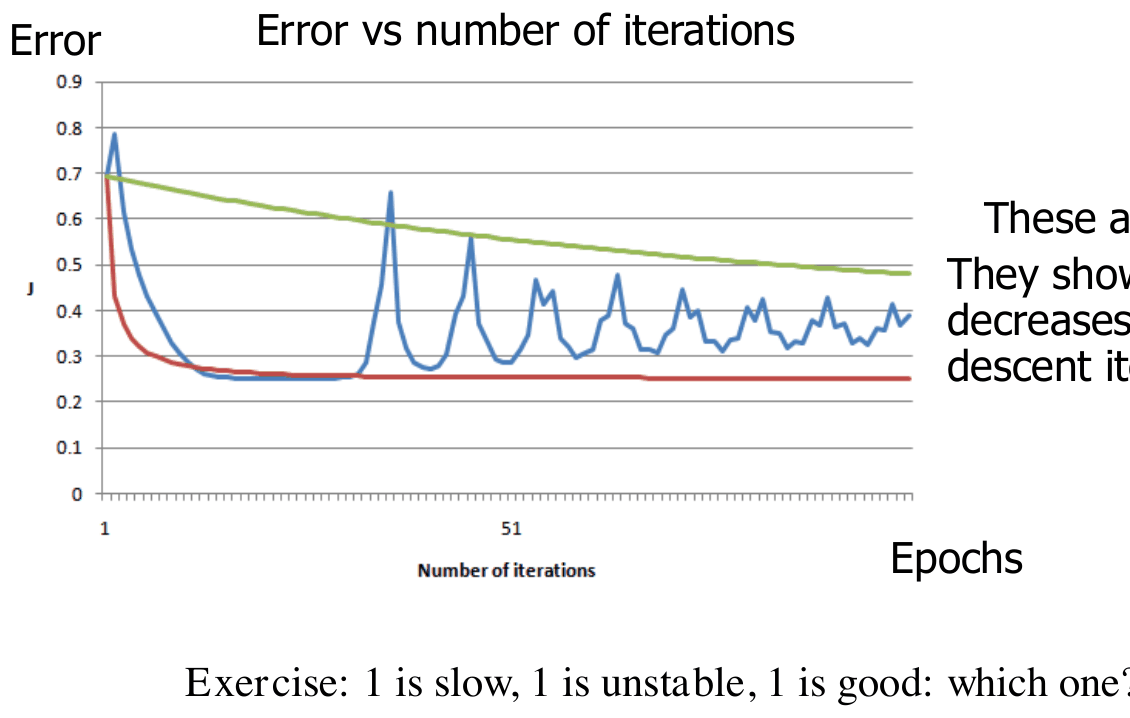
\includegraphics[width=0.63\linewidth,height=0.42\textheight,keepaspectratio]{images/05-lin_curve-apprendimento.png}
\caption{Curve di apprendimento: l'errore in funzione delle iterazioni (epoche).}
\end{figure}

\begin{boxquestion}{Esercizio: quale curva è lenta, quale instabile, quale buona?}

La curva \textbf{verde} scende molto lentamente (learning rate troppo
piccolo); la \textbf{blu} presenta picchi e oscillazioni (learning rate
troppo grande, instabile); la \textbf{rossa} scende rapidamente e si
stabilizza (buona).

\end{boxquestion}

\subsubsection{Interpretazione: una regola di correzione
dell'errore}\label{interpretazione-una-regola-di-correzione-dellerrore}

Ricapitolando, \[
\Delta w_j = 2\sum_{p=1}^{l} \underbrace{(y_p - \mathbf{x}_p^T\mathbf{w})}_{\delta_p}\, x_{p,j}, \qquad \mathbf{w}_{new} = \mathbf{w} + \eta\,\Delta\mathbf{w}
\] (la costante 2 si può omettere, assorbendola in \(\eta\)). È una
regola di \textbf{correzione dell'errore}, detta \textbf{regola di
Widrow-Hoff} o \textbf{delta rule}: ogni \(w_j\) cambia \textbf{in
proporzione all'errore} (target − output).

\begin{itemize}
\tightlist
\item
  Se l'errore è 0, non c'è correzione.
\item
  Con input \(x_j > 0\): se l'errore è positivo (output troppo basso),
  delta positivo → \(w_j\) aumenta → l'output aumenta → l'errore
  diminuisce.
\item
  Con input \(x_j > 0\): se l'errore è negativo (output troppo alto),
  delta negativo → \(w_j\) diminuisce → l'output diminuisce → l'errore
  diminuisce.
\item
  Con input negativo i segni si invertono, con input nullo il peso non
  cambia: l'input ``decide'' quanto e in che verso ogni peso è
  responsabile dell'errore.
\end{itemize}

Si impara dagli errori precedenti: \emph{``cercando e sbagliando si
impara''} (Goethe).

\begin{figure}[htbp]
\centering
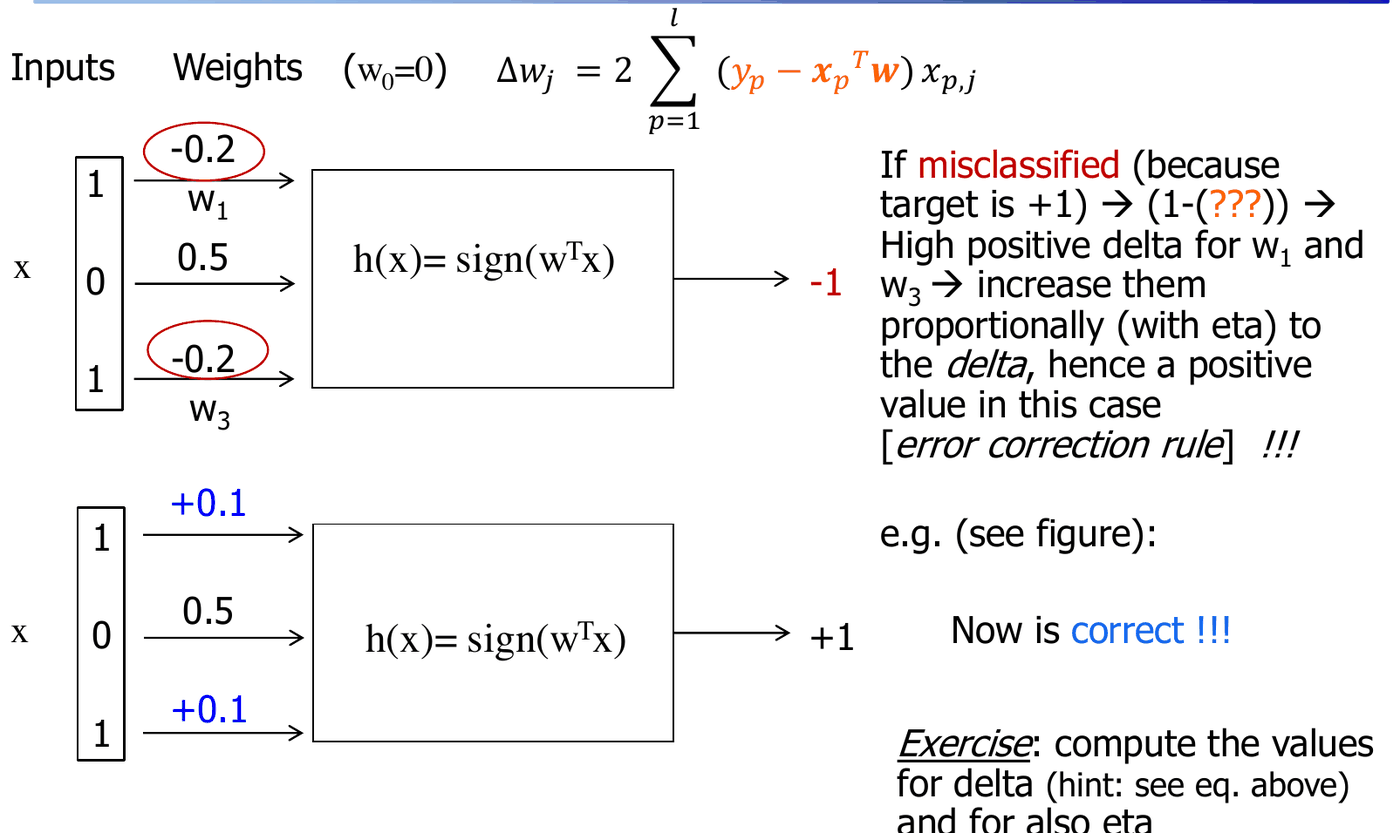
\includegraphics[width=0.86\linewidth,height=0.42\textheight,keepaspectratio]{images/05-lin_delta-rule.png}
\caption{La delta rule all'opera: i pesi degli input attivi vengono aumentati
finché il pattern viene classificato correttamente.}
\end{figure}

Nell'esempio, l'input è \((1, 0, 1)\) con pesi
\((-0{,}2;\ 0{,}5;\ -0{,}2)\) e \(w_0 = 0\):
\(\mathbf{w}^T\mathbf{x} = -0{,}4\), quindi l'uscita è \(-1\) ma il
target è \(+1\). Il delta è positivo: \(w_1\) e \(w_3\) (i cui input
valgono 1) vengono aumentati, mentre \(w_2\) (input 0) resta invariato.
Dopo la correzione (\(w_1 = w_3 = +0{,}1\)) si ha
\(\mathbf{w}^T\mathbf{x} = 0{,}2 > 0\) e l'uscita è corretta.

\begin{boxtip}{Perché la discesa del gradiente è così importante}

È un metodo di ricerca locale semplice ed efficace che permette di
esplorare uno spazio delle ipotesi \textbf{infinito e continuo}. Si
applica sempre quando \(H\) è continuo e la loss è differenziabile,
\textbf{non solo ai modelli lineari}: sarà la base dell'addestramento di
reti neurali e deep learning. Esistono molti miglioramenti (metodi di
Newton e quasi-Newton, gradiente coniugato\ldots).

\end{boxtip}

\subsection{Riepilogo per la
classificazione}\label{riepilogo-per-la-classificazione}

\begin{itemize}
\tightlist
\item
  Il modello viene addestrato sul TR con LMS applicato a
  \(\mathbf{w}^T\mathbf{x}\), tramite la stessa discesa del gradiente
  usata per la regressione.
\item
  Il modello viene \textbf{usato} per classificare applicando la soglia:
  \(h(\mathbf{x}) = \operatorname{sign}(\mathbf{w}^T\mathbf{x})\).
\item
  L'errore si può valutare come \textbf{errore di classificazione} (loss
  0/1, numero di pattern sbagliati), non solo come MSE: \[
  \text{mean\_err} = \frac{1}{l}\sum_{p=1}^{l} L\big(h(\mathbf{x}_p), d_p\big) = \frac{\text{num\_err}}{l}, \qquad \text{accuratezza} = \frac{l - \text{num\_err}}{l}.
  \]
\end{itemize}

\subsection{Torniamo al problema: è una buona
soluzione?}\label{torniamo-al-problema-uxe8-una-buona-soluzione}

\begin{figure}[htbp]
\centering
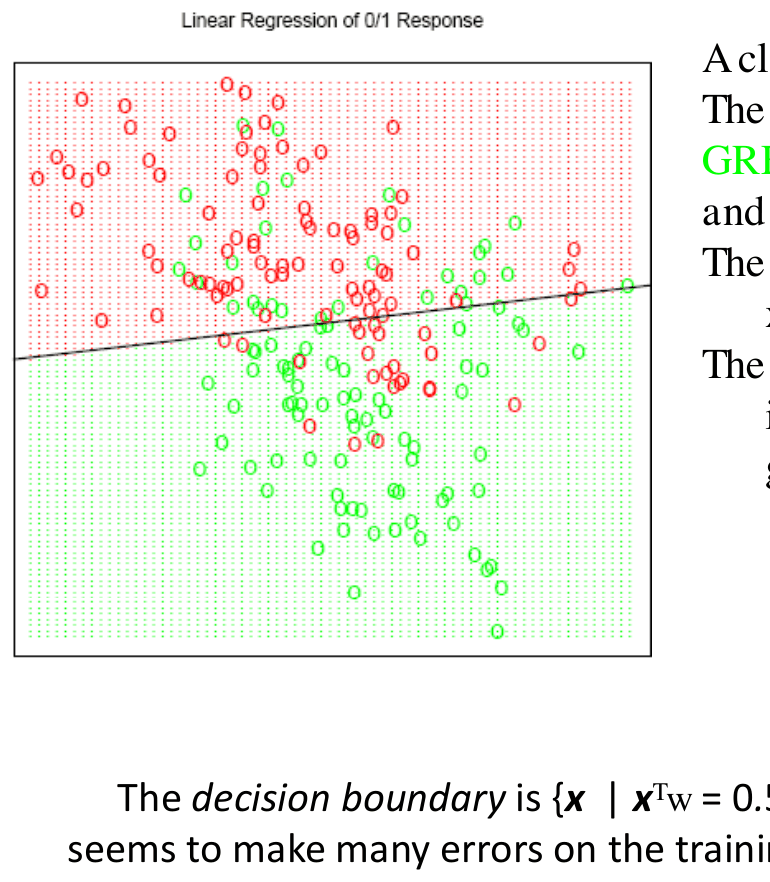
\includegraphics[width=0.46\linewidth,height=0.42\textheight,keepaspectratio]{images/05-lin_htf-lineare.png}
\caption{Soluzione lineare al problema di esempio: classi codificate come GREEN =
0, RED = 1, confine \(\mathbf{x}^T\mathbf{w} = 0{,}5\).}
\end{figure}

Il confine \(\{\mathbf{x} \mid \mathbf{x}^T\mathbf{w} = 0{,}5\}\) è
lineare e sembra commettere molti errori sul training. È una cattiva
soluzione? Dipende da come sono stati generati i dati:

\begin{itemize}
\tightlist
\item
  \textbf{Scenario 1}: ogni classe è generata da una gaussiana con
  componenti scorrelate, stessa varianza e medie diverse. In questo caso
  la regola lineare è \textbf{quasi ottima}: la sovrapposizione tra le
  classi è inevitabile (dovuta al rumore nei dati).
\item
  \textbf{Scenario 2}: ogni classe è una miscela di 10 gaussiane. In
  questo caso il modello lineare è \textbf{troppo rigido}, e servono i
  modelli successivi.
\end{itemize}

\begin{boxnote}{Minimi quadrati e massima verosimiglianza}

I minimi quadrati corrispondono al criterio di \textbf{massima
verosimiglianza} se gli errori sperimentali hanno distribuzione normale.

\end{boxnote}

\subsection{Bias induttivo del modello
lineare}\label{bias-induttivo-del-modello-lineare}

\begin{itemize}
\tightlist
\item
  \textbf{Language bias}: \(H\) è l'insieme delle funzioni lineari, che
  può essere molto restrittivo e rigido.
\item
  \textbf{Search bias}: ricerca ordinata guidata dalla minimizzazione
  dei minimi quadrati. Si potrebbe preferire un metodo diverso, che ad
  esempio restringa i valori dei parametri, ottenendo soluzioni con
  proprietà diverse (in particolare rispetto alla generalizzazione).
\end{itemize}

Anche per un modello ``semplice'' le possibilità sono molte: serve un
approccio fondato su principi (la teoria del ML).

\section{Limiti dei modelli lineari}\label{limiti-dei-modelli-lineari}

\subsection{Regressione di problemi non
lineari}\label{regressione-di-problemi-non-lineari}

Se la funzione target non è lineare (come il seno dell'esempio
polinomiale), una retta è una soluzione \textbf{troppo povera}: è il
caso \(M = 1\) già visto, in piena zona di underfitting.

\subsection{Classificazione: separabilità
lineare}\label{classificazione-separabilituxe0-lineare}

\begin{boxdefinition}{Separabilità lineare}

Due insiemi di punti nel piano sono \textbf{linearmente separabili} se
possono essere separati completamente da una singola retta. In generale,
due gruppi sono linearmente separabili in uno spazio \(n\)-dimensionale
se possono essere separati da un iperpiano di dimensione \(n-1\).

\end{boxdefinition}

Il confine di decisione lineare fornisce soluzioni esatte \textbf{solo}
per insiemi linearmente separabili.

Il modello lineare può rappresentare ad esempio le
\textbf{congiunzioni}. La congiunzione \(x_1 \wedge x_2 \wedge x_4\) si
realizza con
\(1 \cdot x_1 + 1 \cdot x_2 + 0 \cdot x_3 + 1 \cdot x_4 \ge 2{,}5\)
(vale solo se tutti e tre sono 1); l'AND a due variabili con
\(x_1 + x_2 \ge 1{,}5\). I pesi \(\mathbf{w}\) di queste soluzioni
possono essere appresi.

\begin{figure}[htbp]
\centering
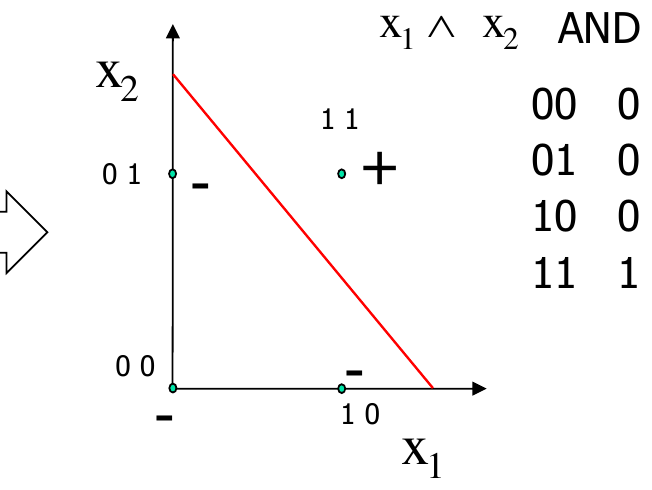
\includegraphics[width=0.40\linewidth,height=0.42\textheight,keepaspectratio]{images/05-lin_and.png}
\caption{L'AND è linearmente separabile.}
\end{figure}

Ma non tutto è separabile:

\begin{itemize}
\tightlist
\item
  \textbf{3 punti}: si può sempre trovare un iperpiano per ogni
  assegnamento delle etichette? Sì, \textbf{se non sono allineati}. Se
  sono allineati, l'etichettatura ``1--0--1'' (0 in mezzo) non è
  separabile.
\item
  \textbf{4 punti}: no. Esiste un'etichettatura per cui nessun
  classificatore lineare è perfetto: lo \textbf{XOR} (\(00 \mapsto 0\),
  \(01 \mapsto 1\), \(10 \mapsto 1\), \(11 \mapsto 0\)), in cui i
  positivi stanno su una diagonale e i negativi sull'altra.
\end{itemize}

\begin{figure}[htbp]
\centering
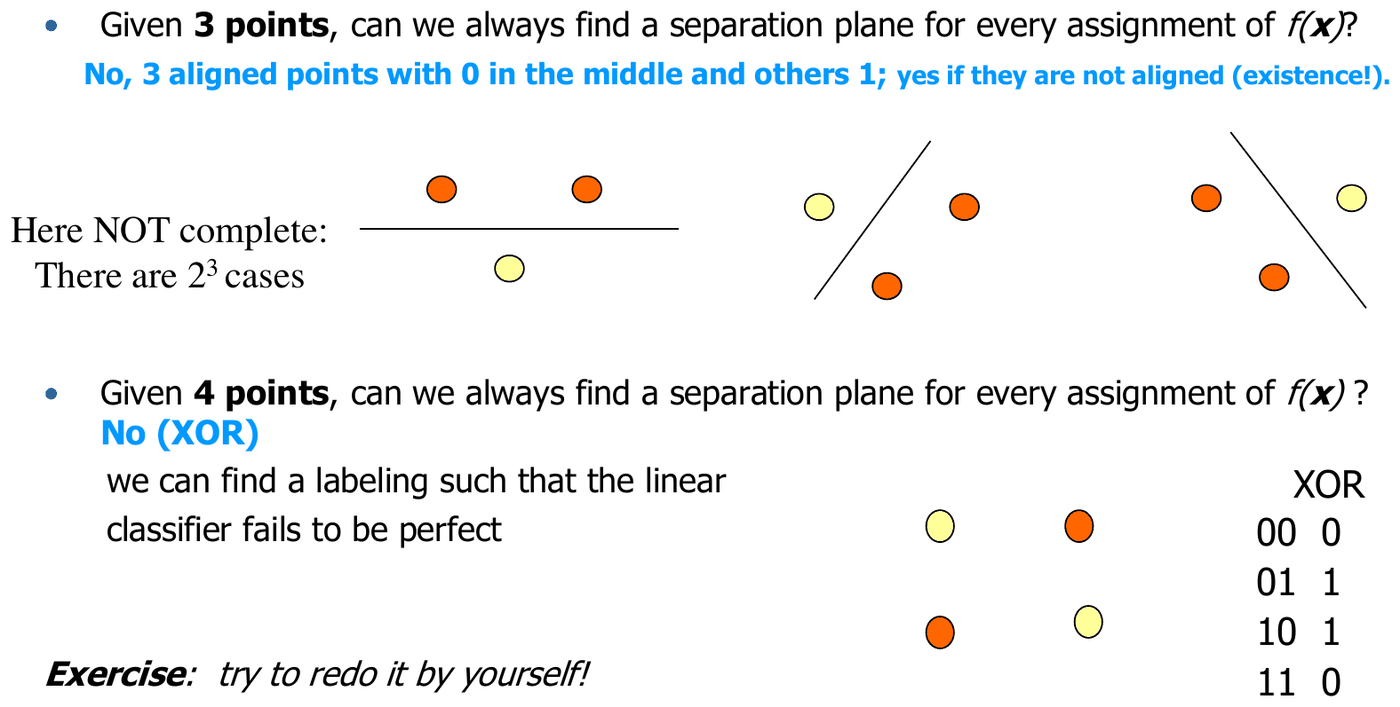
\includegraphics[width=0.86\linewidth,height=0.42\textheight,keepaspectratio]{images/05-lin_xor.png}
\caption{Limiti della separazione lineare: tre punti non allineati sono sempre
separabili, lo XOR su quattro punti no.}
\end{figure}

\begin{boxnote}{Anticipazione}

Questo ``contare quante etichettature si riescono a separare'' è
esattamente l'idea della \textbf{VC-dimension}: un iperpiano nel piano
separa tutte le etichettature di 3 punti (non allineati), ma non di 4.
La VC-dimension delle rette nel piano è quindi 3.

\end{boxnote}

\section{Estendere il modello
lineare}\label{estendere-il-modello-lineare}

\subsection{``Lineare'' nei parametri, non negli
input}\label{lineare-nei-parametri-non-negli-input}

Nei modelli statistici parametrici, \textbf{``lineare'' non si riferisce
alla retta}, ma al modo in cui i \textbf{coefficienti \(\mathbf{w}\)}
compaiono nell'equazione. Si possono quindi usare input trasformati come
\(x, x^2, x^3, \dots\) per modellare relazioni non lineari tra input e
output, mantenendo \textbf{la stessa macchina di apprendimento} (minimi
quadrati). È proprio la regressione polinomiale dell'introduzione: \[
h_\mathbf{w}(x) = w_0 + w_1 x + w_2 x^2 + \dots + w_M x^M = \sum_{j=0}^{M} w_j x^j.
\]

\subsection{Linear Basis Expansion
(LBE)}\label{linear-basis-expansion-lbe}

\begin{boxdefinition}{Espansione in basi lineare}

\[
h_\mathbf{w}(\mathbf{x}) = \sum_{k=0}^{K} w_k\, \phi_k(\mathbf{x})
\] dove le \(\phi_k: \mathbb{R}^n \to \mathbb{R}\) sono trasformazioni
fissate dell'input. Si aumenta il vettore di input con nuove variabili
derivate da \(\mathbf{x}\).

\end{boxdefinition}

Esempi di \(\phi\):

\begin{itemize}
\tightlist
\item
  rappresentazione \textbf{polinomiale}: \(\phi(\mathbf{x}) = x_j^2\),
  \(\phi(\mathbf{x}) = x_j x_i\), \ldots;
\item
  trasformazioni non lineari di singoli input: \(\log(x_j)\),
  \(\sqrt{x_j}\), \ldots;
\item
  trasformazioni di più input: \(\phi(\mathbf{x}) = \|\mathbf{x}\|\);
\item
  spline, \ldots{}
\end{itemize}

Ad esempio:
\(h(\mathbf{x}) = w_1x_1 + w_2x_2 + w_3\log(x_2) + w_4\log(x_3) + w_5(x_2x_3) + w_0\).

Tipicamente il numero di parametri diventa \(K > n\). Il modello è
\textbf{lineare nei parametri} (e nelle \(\phi\)), non in
\(\mathbf{x}\): si usa lo stesso algoritmo di apprendimento. Vale per la
regressione e anche per la classificazione (basta applicare la soglia a
\(\sum_k w_k\phi_k(\mathbf{x})\)).

\begin{boxwarning}{Pro e contro della basis expansion}

\textbf{Pro}: modella relazioni più complesse, è più espressivo.

\textbf{Contro}: - con molte funzioni di base si rischia facilmente
l'\textbf{overfitting}, quindi servono metodi di controllo della
complessità (intesa come flessibilità, cioè VC-dim, non come costo
computazionale); - la \textbf{maledizione della dimensionalità}
(\emph{curse of dimensionality}): il volume dello spazio cresce così in
fretta che i dati disponibili diventano sparsi e non bastano più a
sostenere la complessità del modello; - le \(\phi\) sono \textbf{fissate
prima} di vedere i dati. L'alternativa sono modelli adattivi, non
lineari nei parametri, come le \textbf{reti neurali} (che imparano le
\(\phi\)) e le \textbf{SVM}.

Resta poi aperta la domanda: quali \(\phi\) scegliere? (approcci ``a
dizionario'').

\end{boxwarning}

\section{Regolarizzazione: il controllo della
complessità}\label{regolarizzazione-il-controllo-della-complessituxe0}

Come controllare la complessità del modello? Tra i molti approcci c'è il
\textbf{coefficient shrinkage} (``restringimento'' dei coefficienti).

\subsection{Ridge regression (regolarizzazione di
Tikhonov)}\label{ridge-regression-regolarizzazione-di-tikhonov}

Si aggiunge alla loss un termine che \textbf{penalizza i pesi grandi}:
\[
\text{Loss}(\mathbf{w}) = \underbrace{\sum_{p=1}^{l}(y_p - \mathbf{x}_p^T\mathbf{w})^2}_{\text{termine d'errore (} R_{emp}\text{)}} + \underbrace{\lambda\,\|\mathbf{w}\|^2}_{\text{termine di penalità}}, \qquad \|\mathbf{w}\|^2 = \sum_j w_j^2.
\] \(\lambda\) è l'\textbf{iperparametro di regolarizzazione}, un
piccolo valore positivo scelto in fase di \textbf{model selection}. Il
modello risultante è più ``liscio'' (\emph{smooth}): si favoriscono
modelli con pesi piccoli o nulli, cioè che usano meno termini, quindi
meno complessi.

\begin{boxnote}{Loss ed Errore non sono più sinonimi}

Da qui in poi \textbf{Loss} indica la funzione obiettivo usata per
l'addestramento (errore + penalità), mentre \textbf{Errore} \(E\) indica
la misura dell'errore del modello (il termine sui dati). Finora li
avevamo trattati come equivalenti.

\end{boxnote}

\subsubsection{Soluzione}\label{soluzione}

\begin{itemize}
\tightlist
\item
  \textbf{Approccio diretto}:
  \(\mathbf{w} = (X^TX + \lambda I)^{-1}X^T\mathbf{y}\). La matrice
  \(X^TX + \lambda I\) è \textbf{sempre invertibile} (per
  \(\lambda > 0\)): un vantaggio anche numerico.
\item
  \textbf{Approccio a gradiente}: si segue ancora il gradiente negativo
  della loss. La derivata del termine di penalità rispetto a \(w_j\) è
  \(2\lambda w_j\), quindi la nuova regola è \[
  \mathbf{w}_{new} = \mathbf{w} + \eta\,\Delta\mathbf{w} - 2\lambda\mathbf{w},
  \] dove \(\Delta\mathbf{w}\) è il gradiente negativo del solo termine
  d'errore (moltiplicato per \(\eta\)), mentre la penalità è
  moltiplicata direttamente per \(\lambda\). È la tecnica del
  \textbf{weight decay}: anche con gradiente d'errore nullo, a ogni
  passo ogni peso si riduce di una frazione del suo valore.
\end{itemize}

\subsubsection{\texorpdfstring{Il compromesso governato da
\(\lambda\)}{Il compromesso governato da \textbackslash lambda}}\label{il-compromesso-governato-da-lambda}

\begin{itemize}
\tightlist
\item
  \textbf{\(\lambda\) piccolo}: minimizzando la loss conta soprattutto
  il termine d'errore; si ottiene un modello troppo complesso (pesi di
  norma alta), con rischio di \textbf{overfitting}.
\item
  \textbf{\(\lambda\) grande}: conta soprattutto la penalità; l'errore
  sui dati può crescere troppo, e si va verso l'\textbf{underfitting}.
\end{itemize}

Il grande vantaggio è che si ha una \textbf{realizzazione concreta del
controllo della complessità}, facile da implementare e di applicabilità
generale.

\begin{boxtip}{Tikhonov e SLT}

La penalità spinge tutti i pesi verso valori piccoli (alcuni anche a
zero), realizzando un controllo della complessità: si ottiene un modello
con VC-dimension più bassa (o più adatta), e il compromesso è regolato
da \textbf{un solo parametro}, \(\lambda\). Nel grafico del bound SLT,
aumentare \(\lambda\) equivale a spostarsi verso sinistra (meno
complessità): un \(\lambda\) ben scelto porta vicino al minimo del bound
su \(R\).

\end{boxtip}

\subsubsection{Effetto sul polinomio di grado
9}\label{effetto-sul-polinomio-di-grado-9}

Riprendiamo il polinomio di grado 9 con 10 punti, che senza
regolarizzazione (\(\lambda = 0\)) aveva errore di training nullo e
overfitting fortissimo.

\begin{figure}[htbp]
\centering
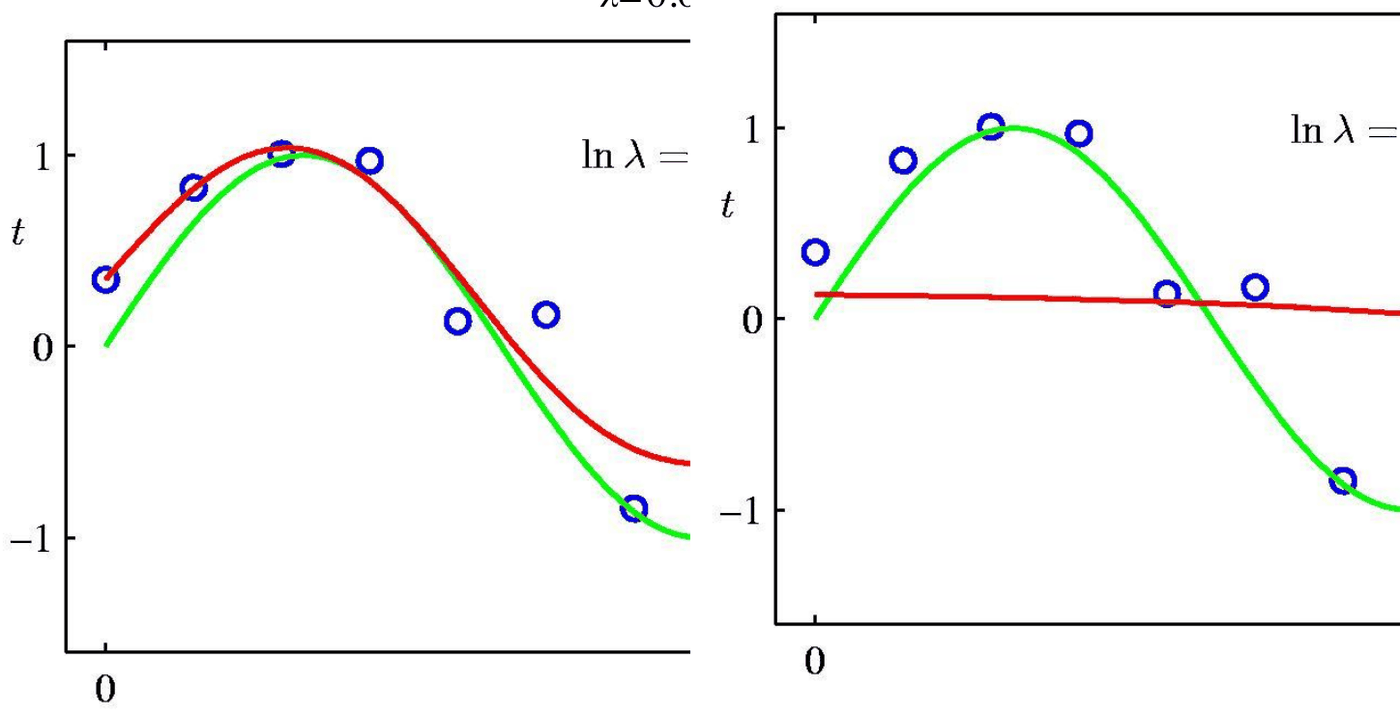
\includegraphics[width=0.80\linewidth,height=0.42\textheight,keepaspectratio]{images/05-lin_regolarizzazione.png}
\caption{Polinomio di grado 9 regolarizzato: con \(\ln\lambda = -18\) (sinistra)
la curva è liscia e segue bene la funzione vera; con \(\ln\lambda = 0\)
(destra) è troppo piatta.}
\end{figure}

Con un \(\lambda\) adatto (\(\ln\lambda = -18\), cioè
\(\lambda \approx 1{,}5 \cdot 10^{-8}\)) il modello funziona bene: è
\textbf{peggiore sul training} ma riduce l'overfitting. Con \(\lambda\)
troppo alto (\(\ln\lambda = 0\), cioè \(\lambda = 1\)) si finisce in
underfitting.

\begin{figure}[htbp]
\centering
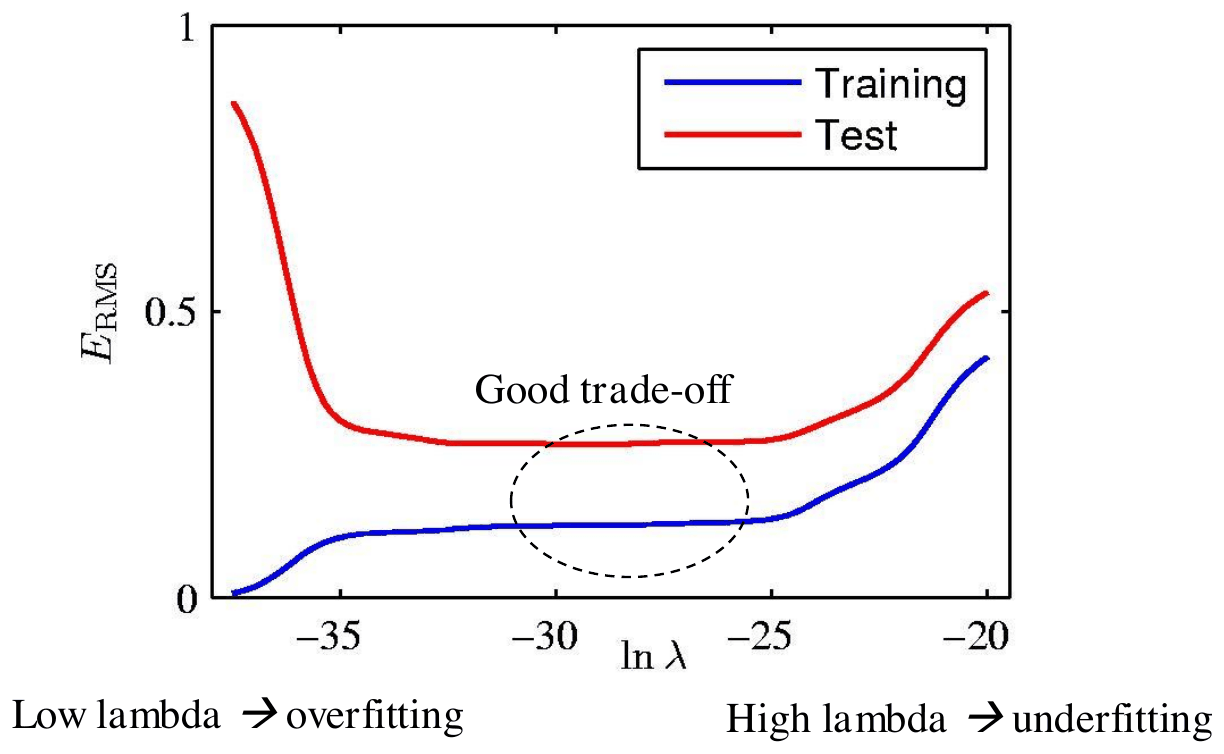
\includegraphics[width=0.63\linewidth,height=0.42\textheight,keepaspectratio]{images/05-lin_rms-lambda.png}
\caption{\(E_{RMS}\) di training e test al variare di \(\ln\lambda\): a sinistra
overfitting, a destra underfitting, al centro il buon compromesso.}
\end{figure}

Anche i coefficienti mostrano l'effetto della regolarizzazione:

{\def\LTcaptype{none} % do not increment counter
\begin{longtable}[]{@{}
  >{\raggedright\arraybackslash}p{(\linewidth - 6\tabcolsep) * \real{0.2500}}
  >{\raggedright\arraybackslash}p{(\linewidth - 6\tabcolsep) * \real{0.2500}}
  >{\raggedright\arraybackslash}p{(\linewidth - 6\tabcolsep) * \real{0.2500}}
  >{\raggedright\arraybackslash}p{(\linewidth - 6\tabcolsep) * \real{0.2500}}@{}}
\toprule\noalign{}
\begin{minipage}[b]{\linewidth}\raggedright
\end{minipage} & \begin{minipage}[b]{\linewidth}\raggedright
\(\ln\lambda = -\infty\) (\(\lambda = 0\))
\end{minipage} & \begin{minipage}[b]{\linewidth}\raggedright
\(\ln\lambda = -18\)
\end{minipage} & \begin{minipage}[b]{\linewidth}\raggedright
\(\ln\lambda = 0\)
\end{minipage} \\
\midrule\noalign{}
\endhead
\bottomrule\noalign{}
\endlastfoot
\(w_0^*\) & 0,35 & 0,35 & 0,13 \\
\(w_1^*\) & 232,37 & 4,74 & −0,05 \\
\(w_2^*\) & −5321,83 & −0,77 & −0,06 \\
\(w_3^*\) & 48568,31 & −31,97 & −0,05 \\
\(w_4^*\) & −231639,30 & −3,89 & −0,03 \\
\(w_5^*\) & 640042,26 & 55,28 & −0,02 \\
\(w_6^*\) & −1061800,52 & 41,32 & −0,01 \\
\(w_7^*\) & 1042400,18 & −45,95 & −0,00 \\
\(w_8^*\) & −557682,99 & −91,53 & 0,00 \\
\(w_9^*\) & 125201,43 & 72,68 & 0,01 \\
\end{longtable}
}

I pesi enormi del caso non regolarizzato si riducono drasticamente: la
regolarizzazione ``doma'' le oscillazioni.

\subsection{Altre tecniche di
regolarizzazione}\label{altre-tecniche-di-regolarizzazione}

\begin{itemize}
\tightlist
\item
  \textbf{Ridge regression} (norma \(\|\cdot\|_2\)): penalizza il
  quadrato dei pesi e tende a rendere \textbf{tutti} i pesi più piccoli.
\item
  \textbf{Lasso} (norma \(\|\cdot\|_1\)): penalizza il valore assoluto e
  tende a portare \textbf{alcuni pesi esattamente a zero} (lasciandone
  altri grandi) → una forma di \textbf{feature selection}. Purtroppo il
  valore assoluto rende la loss non differenziabile (in zero), e servono
  altri approcci.
\item
  \textbf{Elastic net}: usa entrambe le norme.
\end{itemize}

\begin{boxtip}{Perché L1 azzera i pesi e L2 no?}

Il gradiente di \(\lambda w^2\) è \(2\lambda w\): diventa piccolissimo
quando \(w\) è vicino a zero, quindi la spinta verso zero si attenua e
il peso resta piccolo ma non nullo. Il gradiente (sub-gradiente) di
\(\lambda|w|\) è invece \(\lambda\operatorname{sign}(w)\): una spinta
\textbf{costante} verso zero, anche per pesi già piccoli, che li porta
esattamente a zero se il termine d'errore non li ``difende''.

\end{boxtip}

\subsection{Altri miglioramenti
(opzionali)}\label{altri-miglioramenti-opzionali}

\begin{itemize}
\tightlist
\item
  \textbf{Data augmentation}: aggiungere rumore agli input insegna al
  modello a ignorare variazioni irrilevanti (robustezza e
  regolarizzazione); l'oversampling aiuta con dataset sbilanciati.
\item
  \textbf{Input derivati}: si usa un piccolo numero di nuove variabili,
  combinazioni lineari degli input (Principal Component Regression,
  Partial Least Squares).
\end{itemize}

\subsection{Classificazione multi-classe
(opzionale)}\label{classificazione-multi-classe-opzionale}

Due approcci semplici:

\begin{itemize}
\tightlist
\item
  codifica \textbf{1-of-K} delle classi (es. rosso, verde, blu →
  \((0,0,1), (0,1,0), (1,0,0)\)) e un modello lineare per ciascuna
  componente;
\item
  \textbf{OVA} (\emph{one-vs-all}): si addestrano \(K\) classificatori
  binari, ognuno distingue una classe da tutte le altre; per
  classificare si sceglie quello con l'uscita più alta (più positiva);
\item
  \textbf{AVA} (\emph{all-vs-all}, \emph{one-vs-one}): un classificatore
  per ogni coppia di classi (\(K(K-1)/2\) classificatori distinti);
  vince la classe con la massima somma di uscite o con più voti. Ogni
  classificatore si addestra su meno dati.
\end{itemize}

Con molte classi possono verificarsi fenomeni di \textbf{mascheramento}
(una classe ``nascosta'' dalle altre). Esistono approcci più sofisticati
e modelli con uscite multiple native. Altri classificatori lineari noti
sono la \textbf{Linear Discriminant Analysis} e la \textbf{regressione
logistica} (che modella direttamente \(P(y \mid \mathbf{x})\)).

\subsection{Uno sguardo avanti}\label{uno-sguardo-avanti}

\begin{itemize}
\tightlist
\item
  Il \textbf{Perceptron} (Rosenblatt, 1958, di ispirazione biologica)
  minimizza solo le classificazioni errate ed è la base delle
  \textbf{reti neurali}: più unità organizzate in strati, che realizzano
  un'\textbf{espansione in basi adattiva} (le \(\phi\) vengono apprese),
  cioè \emph{representation learning}, addestrate con la discesa del
  gradiente.
\item
  Le \textbf{SVM} (Vapnik, 1996) regolarizzano tramite la
  \textbf{massimizzazione del margine} tra le classi e allargano lo
  spazio delle feature con basis expansion (es. polinomi).
\end{itemize}

Entrambe realizzano un'approssimazione non lineare flessibile per
classificazione e regressione.

\begin{boxabstract}{Lezioni apprese dai modelli lineari}

\begin{itemize}
\tightlist
\item
  È possibile \textbf{apprendere regolando parametri liberi}
  \(\mathbf{w}\), cercando in uno spazio continuo guidati da una
  funzione di loss.
\item
  Si formula il problema come \textbf{LMS} e si derivano due algoritmi:
  \textbf{diretto} (equazioni normali, SVD) e \textbf{iterativo}
  (discesa del gradiente, delta rule).
\item
  I modelli lineari hanno un forte \textbf{language bias} (solo problemi
  linearmente separabili).
\item
  Due concetti chiave del filo rosso del corso: la \textbf{basis
  expansion} (più \textbf{flessibilità}) e la \textbf{regolarizzazione}
  (\textbf{controllo della complessità}). Li ritroveremo, in forme
  diverse, nelle reti neurali e nelle SVM.
\end{itemize}

\end{boxabstract}

\section{K-nearest neighbors}\label{k-nearest-neighbors}

Ora ci si sposta all'estremo opposto: da un approccio rigido a uno
\textbf{molto flessibile} (e locale).

\subsection{Apprendimento eager e
lazy}\label{apprendimento-eager-e-lazy}

Rispetto al \emph{timing} dell'apprendimento distinguiamo:

\begin{itemize}
\tightlist
\item
  \textbf{eager} (``avido''): si analizzano i dati di training e si
  costruisce un'\textbf{ipotesi esplicita} (come il modello lineare);
\item
  \textbf{lazy} (``pigro''): si memorizzano i dati e si aspetta un punto
  di test; solo allora si costruisce un'ipotesi ad hoc per classificare
  quel punto.
\end{itemize}

\subsection{1-nearest neighbor}\label{nearest-neighbor}

\begin{boxdefinition}{Algoritmo 1-NN}

\begin{enumerate}
\def\labelenumi{\arabic{enumi}.}
\tightlist
\item
  Memorizzare i dati di training \(\langle \mathbf{x}_p, y_p\rangle\),
  \(p = 1,\dots,l\).
\item
  Dato un input \(\mathbf{x}\) (di dimensione \(n\)), trovare l'esempio
  di training più vicino: \[
  i(\mathbf{x}) = \arg\min_p d(\mathbf{x}, \mathbf{x}_p),
  \] ad esempio con la distanza euclidea
  \(d(\mathbf{x}, \mathbf{x}_p) = \sqrt{\sum_{t=1}^{n}(x_t - x_{p,t})^2} = \|\mathbf{x} - \mathbf{x}_p\|\).
\item
  Restituire \(y_i\).
\end{enumerate}

\end{boxdefinition}

Il 1-NN è \textbf{molto flessibile}: sul training set commette
\textbf{zero errori} (ogni punto è il vicino più prossimo di sé stesso).
Il confine di decisione non è lineare ed è molto irregolare, forse
inutilmente rumoroso (ad esempio nello scenario 1, dove sappiamo che la
soluzione ottima è quasi lineare). E sui dati di test?

\subsection{K-nearest neighbors}\label{k-nearest-neighbors-1}

Un modo naturale di classificare un nuovo punto è guardare i suoi
\textbf{vicini} e farne la media: \[
\text{avg}_k(\mathbf{x}) = \frac{1}{k}\sum_{\mathbf{x}_i \in N_k(\mathbf{x})} y_i,
\] dove \(N_k(\mathbf{x})\) è l'insieme dei \(k\) pattern più vicini a
\(\mathbf{x}\) secondo la distanza \(d\). Se nell'intorno di
\(\mathbf{x}\) una classe domina chiaramente, è probabile che anche
\(\mathbf{x}\) vi appartenga: la regola di classificazione è il
\textbf{voto a maggioranza} tra i membri di \(N_k(\mathbf{x})\). Per
target in \(\{0,1\}\): \[
h(\mathbf{x}) = \begin{cases} 1 & \text{se } \text{avg}_k(\mathbf{x}) > 0{,}5 \\ 0 & \text{altrimenti.} \end{cases}
\] Per la \textbf{regressione} si usa direttamente la media dei target
dei \(k\) vicini.

\begin{figure}[htbp]
\centering
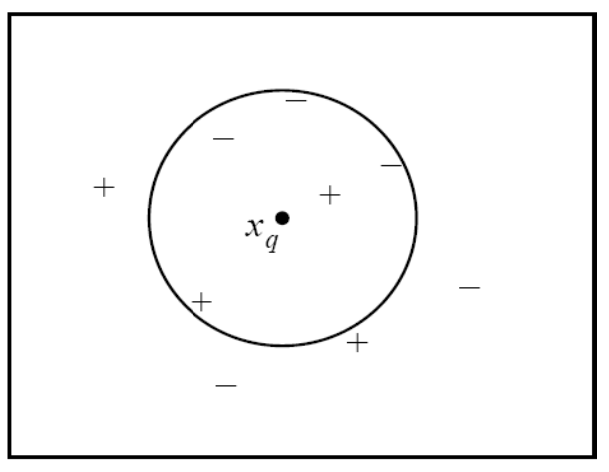
\includegraphics[width=0.34\linewidth,height=0.42\textheight,keepaspectratio]{images/05-knn_1nn-vs-5nn.png}
\caption{1-NN restituisce ``+'' per \(x_q\), 5-NN restituisce ``−'': aumentare
\(k\) ``liscia'' la decisione, utile con dati rumorosi.}
\end{figure}

\begin{figure}[htbp]
\centering
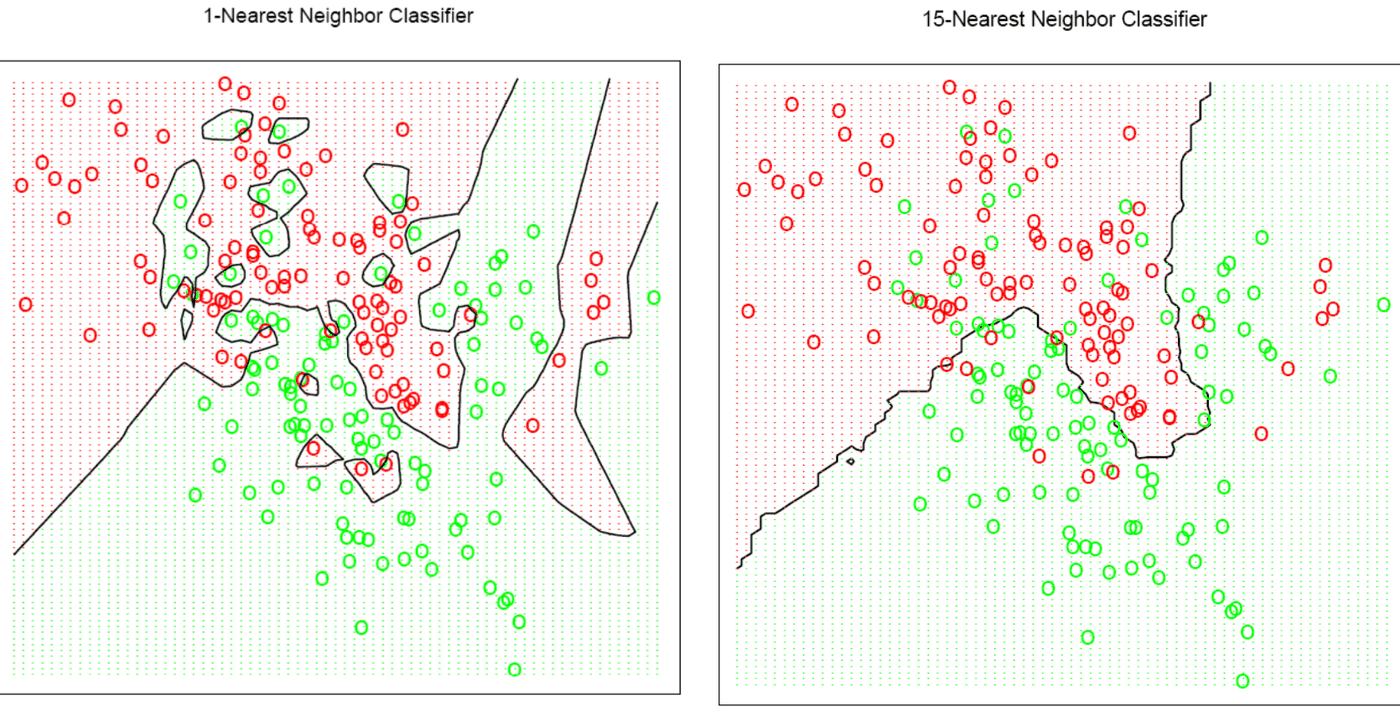
\includegraphics[width=0.89\linewidth,height=0.42\textheight,keepaspectratio]{images/05-knn_1nn-15nn.png}
\caption{Confini di decisione del 1-NN (sinistra) e del 15-NN (destra) sullo
stesso problema.}
\end{figure}

Con \(k = 15\) il modello è ancora molto flessibile, ma commette qualche
errore sul training; il confine è ancora irregolare ma meno, e si
\textbf{adatta alle densità locali} delle classi.

Il K-NN usa implicitamente il \textbf{diagramma di Voronoi}: ogni cella
contiene tutti i punti più vicini a un certo pattern che a qualsiasi
altro, e i lati delle celle sono i punti equidistanti da due pattern. Il
1-NN assegna a ogni cella l'etichetta del suo pattern.

\begin{figure}[htbp]
\centering
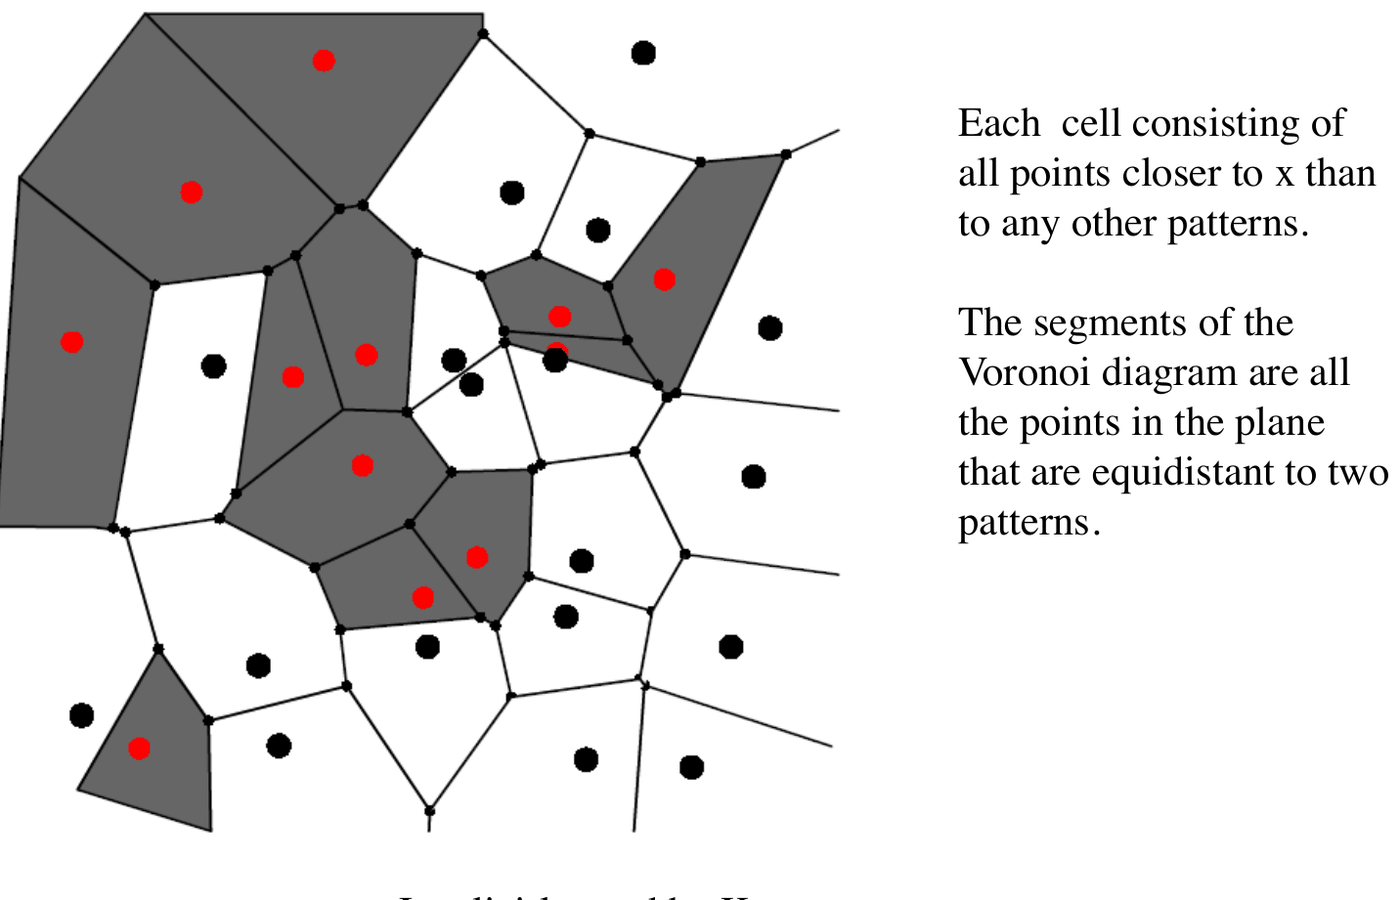
\includegraphics[width=0.69\linewidth,height=0.42\textheight,keepaspectratio]{images/05-knn_voronoi.png}
\caption{Diagramma di Voronoi: il confine del 1-NN segue i lati delle celle tra
punti di classi diverse.}
\end{figure}

\subsection{Varianti}\label{varianti}

\textbf{Multi-classe}: si restituisce la classe più frequente tra i
\(k\) vicini: \[
h(\mathbf{x}) = \arg\max_v \sum_{\mathbf{x}_i \in N_k(\mathbf{x})} \mathbb{1}_{v, y_i}, \qquad \mathbb{1}_{v, y_i} = \begin{cases} 1 & \text{se } v = y_i \\ 0 & \text{altrimenti.} \end{cases}
\]

\textbf{Distanza pesata}: i vicini più vicini contano di più: \[
h(\mathbf{x}) = \arg\max_v \sum_{\mathbf{x}_i \in N_k(\mathbf{x})} \frac{\mathbb{1}_{v, y_i}}{d(\mathbf{x}, \mathbf{x}_i)^2},
\] e se \(d = 0\) per qualche \(\mathbf{x}_i\) si restituisce
direttamente \(y_i\).

\subsection{Un estremo del ML}\label{un-estremo-del-ml}

Il K-NN non costruisce un'ipotesi globale valida per tutte le istanze:
\textbf{non c'è un modello da addestrare}, ma bisogna memorizzare gli
esempi. Fa stime \textbf{locali} (con funzioni localmente costanti)
invece di un'approssimazione lineare globale. È un metodo \emph{lazy},
basato su memoria, sulle istanze, sulle distanze.

\subsection{K-NN contro modello
lineare}\label{k-nn-contro-modello-lineare}

{\def\LTcaptype{none} % do not increment counter
\begin{longtable}[]{@{}
  >{\raggedright\arraybackslash}p{(\linewidth - 4\tabcolsep) * \real{0.3333}}
  >{\raggedright\arraybackslash}p{(\linewidth - 4\tabcolsep) * \real{0.3333}}
  >{\raggedright\arraybackslash}p{(\linewidth - 4\tabcolsep) * \real{0.3333}}@{}}
\toprule\noalign{}
\begin{minipage}[b]{\linewidth}\raggedright
\end{minipage} & \begin{minipage}[b]{\linewidth}\raggedright
Lineare
\end{minipage} & \begin{minipage}[b]{\linewidth}\raggedright
K-NN
\end{minipage} \\
\midrule\noalign{}
\endhead
\bottomrule\noalign{}
\endlastfoot
Flessibilità & rigido (\textbf{bassa varianza}) & flessibile
(\textbf{alta varianza}) \\
Timing & eager & lazy \\
Tipo & parametrico & instance-based \\
Parametri & \(n+1\) (3 nell'esempio) & circa \(l/k\) ``parametri
effettivi'' \\
\end{longtable}
}

Con \(k\) piccolo bastano pochi punti per cambiare il confine: la
flessibilità si paga. Si potrebbe pensare che il K-NN abbia un solo
parametro (\(k\)), ma realisticamente ha circa \textbf{\(l/k\) parametri
effettivi} (Hastie-Tibshirani-Friedman): è come se dividesse lo spazio
in \(l/k\) regioni, ognuna con la sua ``media''.

\begin{figure}[htbp]
\centering
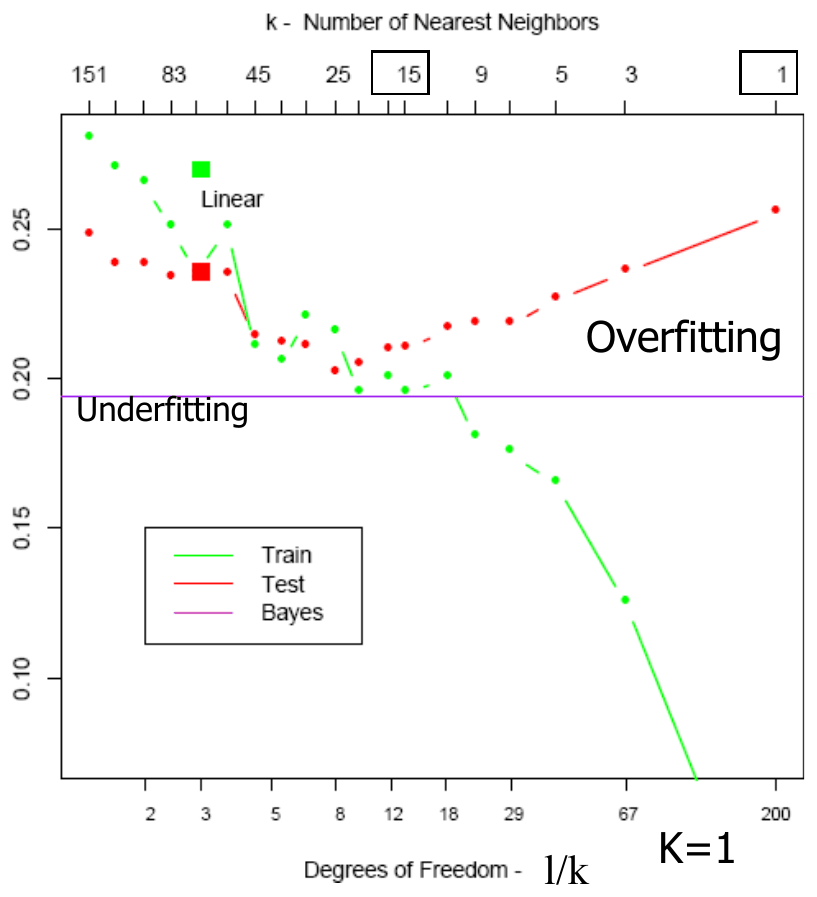
\includegraphics[width=0.54\linewidth,height=0.42\textheight,keepaspectratio]{images/05-knn_errori-k.png}
\caption{Curve di errore del K-NN al variare di \(k\) (training di 200 punti,
test di 10000). I quadratini sono il modello lineare, la linea viola
l'errore ottimo di Bayes.}
\end{figure}

Spostandosi da \(k\) grande a \(k = 1\) (cioè aumentando \(l/k\)) si
passa dall'\textbf{underfitting} all'\textbf{overfitting}: l'errore di
training scende fino a zero, quello di test ha un minimo per valori
intermedi. È di nuovo il grafico del bound SLT, con \(k\) nel ruolo del
controllo della complessità: più flessibilità permette di trovare il
risultato migliore, \textbf{se} la complessità viene controllata.

\subsection{Il classificatore ottimo di
Bayes}\label{il-classificatore-ottimo-di-bayes}

\begin{boxdefinition}{Classificatore di Bayes ed errore di Bayes}

Se si conosce la densità \(P(\mathbf{x}, y)\), la scelta ottima è
assegnare la classe più probabile: \[
h(\mathbf{x}) = \arg\max_v P(v \mid \mathbf{x}), \qquad v \in \{C_1, \dots, C_K\}.
\] Il suo tasso d'errore, detto \textbf{Bayes rate}, è il \textbf{minimo
errore raggiungibile} data la distribuzione dei dati (assumendo nota la
densità generatrice).

\end{boxdefinition}

Il K-NN approssima direttamente questa soluzione: il voto a maggioranza
in un intorno è esattamente una stima di
\(\arg\max_v P(v \mid \mathbf{x})\), con due rilassamenti: la
probabilità condizionata \textbf{in un punto} diventa probabilità
condizionata \textbf{in un intorno} del punto (approssimazione locale),
e le probabilità sono stimate con le \textbf{proporzioni} nel campione
di training.

\begin{figure}[htbp]
\centering
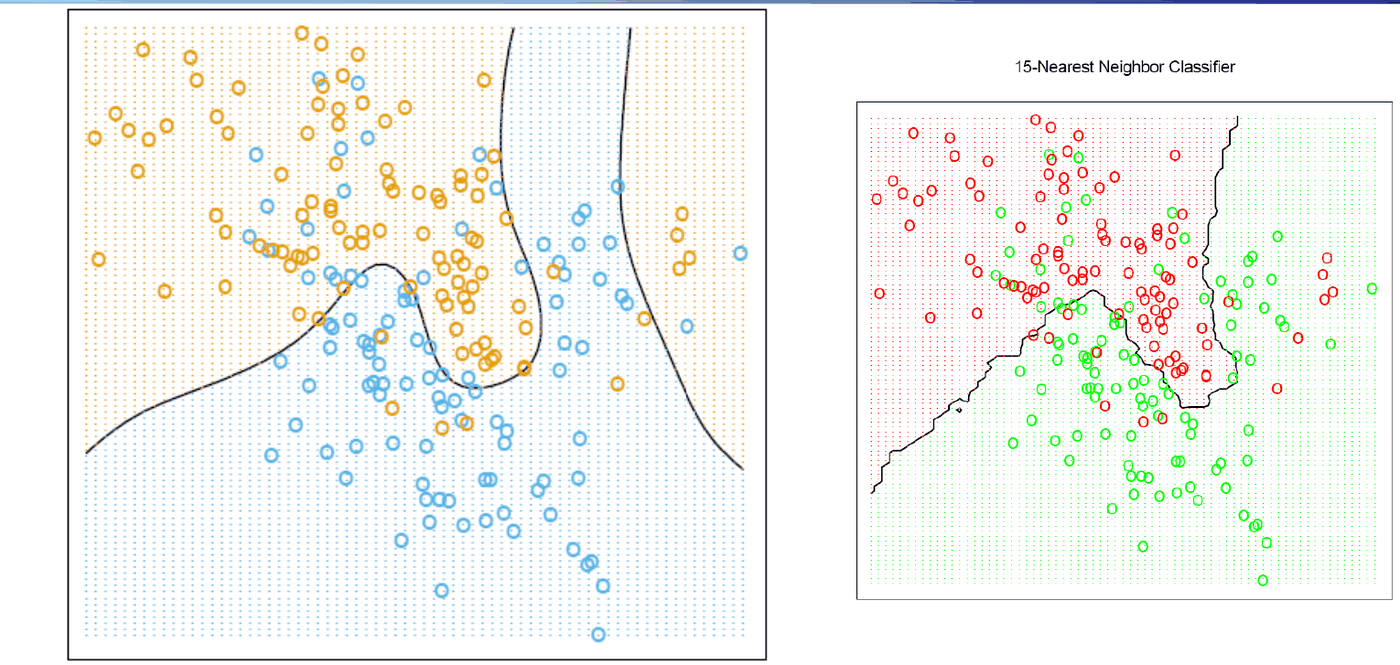
\includegraphics[width=0.80\linewidth,height=0.42\textheight,keepaspectratio]{images/05-knn_bayes.png}
\caption{Confine di Bayes ottimo (sinistra) e confine del 15-NN (destra): il
15-NN è molto vicino all'ottimo, coerentemente con il minimo dell'errore
di test nella figura precedente.}
\end{figure}

\subsection{Bias induttivo del K-NN}\label{bias-induttivo-del-k-nn}

\begin{enumerate}
\def\labelenumi{\arabic{enumi}.}
\tightlist
\item
  \textbf{La distanza assunta} stabilisce quali esempi sono simili: si
  assume che la classificazione di un punto sia simile a quella dei
  vicini \textbf{secondo la metrica scelta}. Si possono usare metriche
  diverse dall'euclidea; dati simbolici richiedono metriche ad hoc (es.
  la \textbf{distanza di Hamming} tra stringhe della stessa lunghezza:
  il numero di posizioni in cui differiscono).
\item
  \textbf{Località}: approssimazione locale, con un'assunzione di
  \emph{smoothness} locale (da confrontare più avanti con il bias del
  deep learning).
\end{enumerate}

Il bias legato alla metrica è spesso sottovalutato nei libri, ma è
cruciale.

\subsection{Limiti del K-NN}\label{limiti-del-k-nn}

\subsubsection{Scala delle variabili e
metrica}\label{scala-delle-variabili-e-metrica}

La scelta della scala dipende dalla conoscenza del dominio. Se le
variabili devono contribuire allo stesso modo, bisogna fare attenzione
alle differenze di range: \textbf{riscalare i dati} (es. media zero e
varianza unitaria) equivale a \textbf{cambiare la metrica}. La scalatura
può cambiare del tutto quale sia il vicino più prossimo: il K-NN è
fragile anche rispetto a un pre-processing elementare.

\begin{figure}[htbp]
\centering
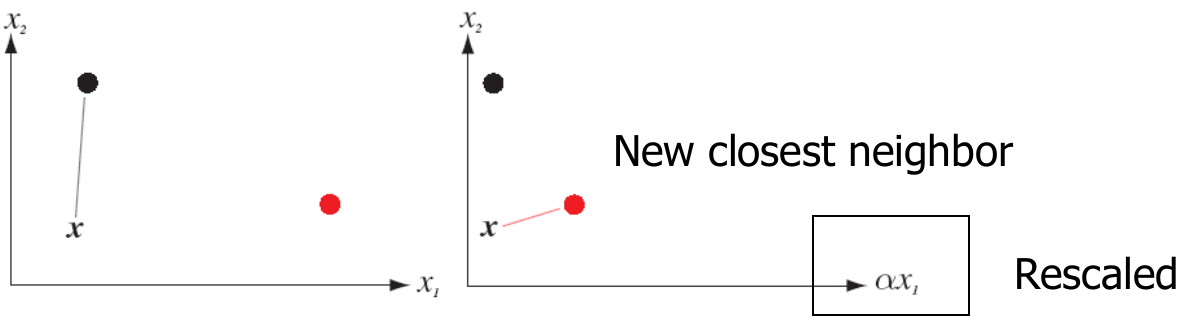
\includegraphics[width=0.71\linewidth,height=0.42\textheight,keepaspectratio]{images/05-knn_scala.png}
\caption{Riscalando una variabile cambia il vicino più prossimo.}
\end{figure}

\subsubsection{Costo computazionale}\label{costo-computazionale}

Il K-NN costruisce l'approssimazione locale \textbf{per ogni nuovo
esempio} da predire: il costo computazionale è \textbf{spostato nella
fase di predizione}. Per ogni input si calcolano le distanze da tutti i
vettori memorizzati (tempo proporzionale al numero di pattern), anche se
esistono algoritmi di ricerca di prossimità e indicizzazione ad hoc.
Anche il costo in \textbf{spazio} è alto (tutti i dati di training).

\subsubsection{Interpretabilità}\label{interpretabilituxe0}

I modelli K-NN offrono poca interpretazione, soggettiva e dipendente
dalla metrica.

\subsubsection{La maledizione della
dimensionalità}\label{la-maledizione-della-dimensionalituxe0}

Il K-NN funziona bene se si trova un insieme significativo di dati
vicini a ogni \(\mathbf{x}\), cioè con un \textbf{campionamento denso}.
Quando ci sono molte variabili di input (dimensione \(n\) alta) fallisce
spesso per la \textbf{curse of dimensionality}, che ha molte
manifestazioni. Tre in particolare influenzano direttamente la
generalizzazione.

\textbf{1. In alta dimensione è difficile trovare punti vicini.} Diventa
difficile raccogliere \(k\) osservazioni ``vicine'' (cioè simili) a un
punto di query: gli intorni tendono a essere spazialmente grandi e le
stime non sono più locali; ridurre la dimensione dell'intorno significa
ridurre \(k\), e la varianza della stima aumenta (overfitting).

Consideriamo dati uniformi nel cubo unitario e un sottocubo che deve
contenere una frazione \(r\) dei dati. Il suo lato deve essere
\(r^{1/n}\) (perché volume \(=\) lato\(^n\)).

\begin{figure}[htbp]
\centering
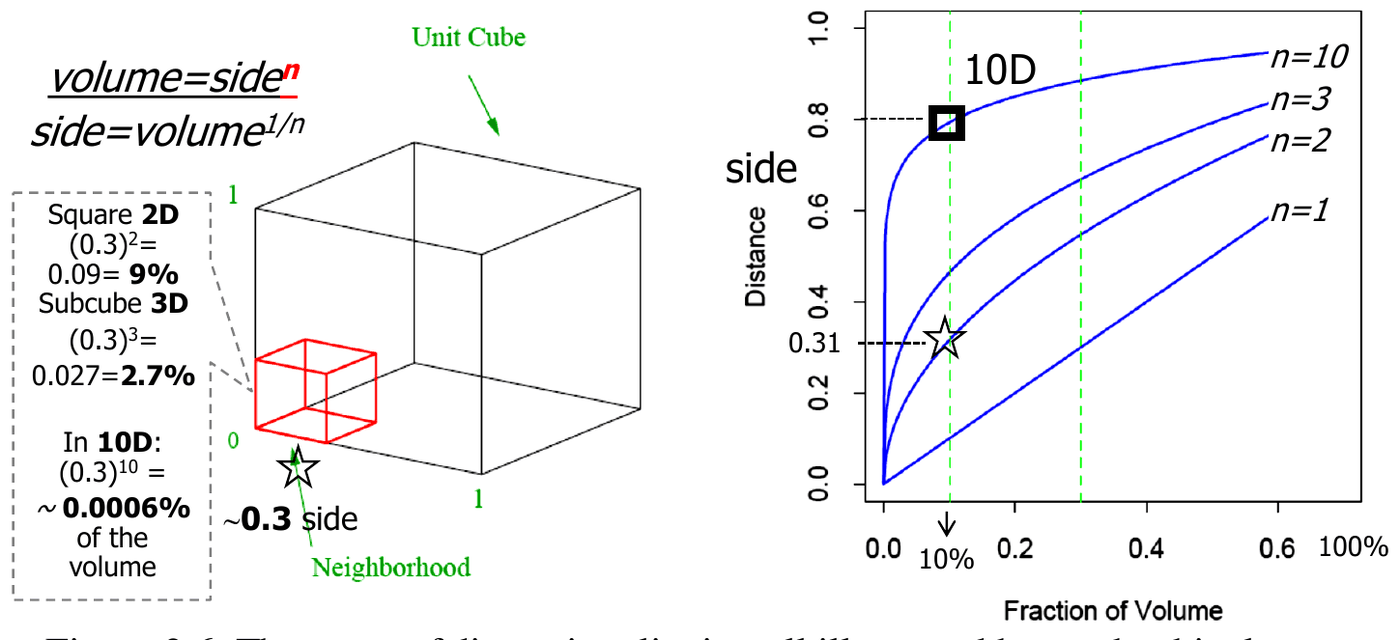
\includegraphics[width=0.86\linewidth,height=0.42\textheight,keepaspectratio]{images/05-knn_curse.png}
\caption{Maledizione della dimensionalità: lato del sottocubo necessario per
catturare una frazione \(r\) del volume, al variare della dimensione
\(n\).}
\end{figure}

\begin{itemize}
\tightlist
\item
  Per catturare il 10\% dei dati: in 2D basta un lato di
  \(0{,}1^{1/2} \approx 0{,}32\) (il 30\% del range di ogni variabile);
  in 10D serve \(0{,}1^{1/10} \approx 0{,}8\), cioè l'\textbf{80\% del
  range} di ogni coordinata! Anche per l'1\% del volume in 10D serve il
  63\% del range. L'intorno non è più ``locale'' e i vicini non sono più
  simili.
\item
  Viceversa, fissato il lato a 0,3: in 1D si cattura il 30\% dei dati,
  in 2D il 9\%, in 3D il 2,7\%, in 10D circa lo \textbf{0,0006\%}. Quel
  lato può non bastare a trovare \(k\) dati, a meno di usare \(k\)
  piccolo (e quindi rischiare overfitting).
\end{itemize}

\textbf{2. Bassa densità di campionamento.} La densità di campionamento
è proporzionale a \(l^{1/n}\). Se 100 punti bastano a stimare una
funzione in \(\mathbb{R}^1\), per ottenere un'accuratezza simile in
\(\mathbb{R}^{10}\) ne servono \(100^{10} = 10^{20}\).

\textbf{3. Feature irrilevanti} (\emph{curse of noisy}). Se il target
dipende solo da poche delle molte feature (es. 2 su 20), la somiglianza
tra pattern può essere dominata dal gran numero di feature irrilevanti,
e il ``vicino'' trovato non è davvero simile. Il problema cresce con la
dimensionalità. Rimedi: \textbf{pesare le feature} secondo la loro
rilevanza (allungando gli assi lungo alcune dimensioni; i pesi si
possono cercare con una costosa model selection o altri metodi) oppure
fare \textbf{feature selection} (eliminare variabili, riducendo la
dimensione dell'input).

\subsection{Scelte di progetto del
K-NN}\label{scelte-di-progetto-del-k-nn}

\begin{itemize}
\tightlist
\item
  La \textbf{metrica} \(d\) (euclidea, Hamming, Manhattan, pesi sulle
  feature\ldots): spesso è la chiave del successo di un'applicazione.
\item
  Il valore di \textbf{\(k\)}, che controlla underfitting e overfitting.
\item
  Spesso è necessario selezionare un \textbf{sottoinsieme dei dati} (un
  insieme di prototipi, ad esempio tramite clustering) e un
  \textbf{sottoinsieme delle feature}.
\end{itemize}

Estensioni ad altri modelli locali: \emph{kernel smoothers}, regressione
lineare locale, metodi a prototipi, \emph{case-based reasoning}.

\begin{boxabstract}{Lezioni generali dal K-NN}

\begin{itemize}
\tightlist
\item
  Una varianza troppo bassa è povera (modelli lineari rigidi), una
  troppo alta è pericolosa (K-NN).
\item
  \textbf{Smoothing}: nel K-NN si ottiene aumentando \(k\).
\item
  \textbf{Curse of dimensionality}: il volume dello spazio cresce così
  in fretta che i dati diventano sparsi.
\item
  Le curve di errore al variare di \(k\) sono un'altra istanza del
  grafico del bound SLT.
\item
  Il bias induttivo del K-NN è legato alla metrica.
\end{itemize}

\end{boxabstract}

\subsection{E adesso?}\label{e-adesso}

Il K-NN non costruisce un vero ``modello appreso'': non estrae
regolarità né sintetizza conoscenza, e non soddisfa l'obiettivo
dell'apprendimento (poter ``dimenticare'' gli esempi dopo aver costruito
il modello). Nelle prossime lezioni si cercano modelli \textbf{compatti}
come la LTU (tutta la conoscenza in pochi parametri) ma
\textbf{flessibili} come il K-NN, con un adeguato supporto al controllo
della complessità: le \textbf{reti neurali}.

\begin{boxquestion}{Possibili domande d'esame}

\begin{itemize}
\tightlist
\item
  Formulare il problema di apprendimento per un modello lineare con LMS,
  per regressione e classificazione.
\item
  Derivare il gradiente dell'errore quadratico e le equazioni normali.
\item
  Descrivere l'algoritmo di discesa del gradiente; differenza tra batch
  e on-line; ruolo di \(\eta\).
\item
  Spiegare la delta rule come regola di correzione dell'errore.
\item
  Perché per la classificazione si usa l'errore quadratico su
  \(\mathbf{w}^T\mathbf{x}\) invece della loss 0/1?
\item
  Cos'è la separabilità lineare? Perché lo XOR non è linearmente
  separabile?
\item
  Cos'è la linear basis expansion? Pro e contro.
\item
  Scrivere la loss di Tikhonov, la soluzione diretta e la regola di
  weight decay; ruolo di \(\lambda\).
\item
  Differenza tra regolarizzazione L1 e L2.
\item
  Descrivere il K-NN; confrontarlo con il modello lineare; cos'è il
  classificatore di Bayes?
\item
  Spiegare la maledizione della dimensionalità.
\end{itemize}

\end{boxquestion}
